\chapter{Data and Simulation Comparison Plots}\label{app:plots}
This appendix contains a selection of comparison plots between data and simulation for the signal region and the \ttbar and Z+jets 0-bjet control regions.
For the signal region and Z+jets control region sections, the left-hand side plots correspond to the $ee$ channel and the right-hand side plots to the $\mu\mu$ channel.

\section{Signal Region}\label{appSec:signalRegionPlots}

\begin{figure}[h]
\centering
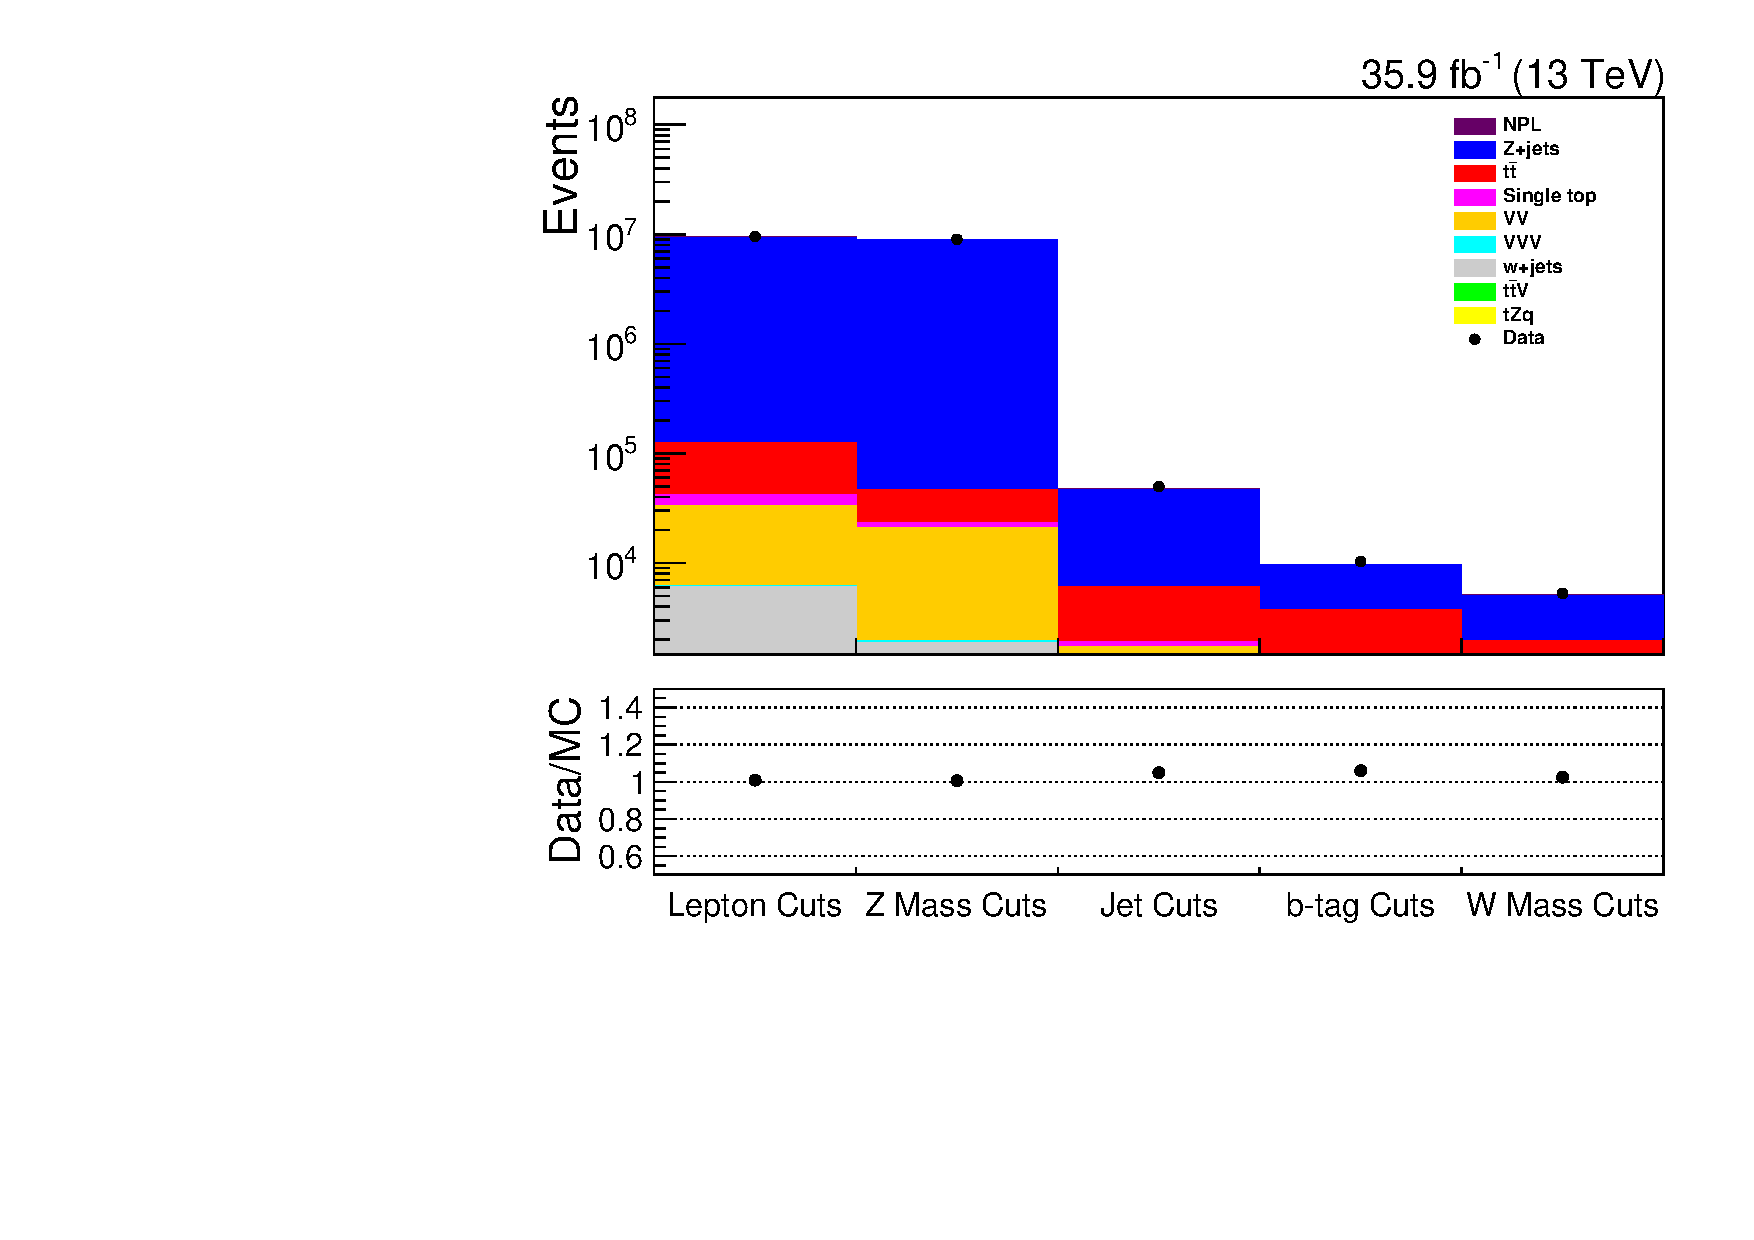
\includegraphics[width=0.97\textwidth]{figs/background-estimation/plots/unblinded/prompt_ee_ttbarInc/cutFlow_log.pdf}
\\
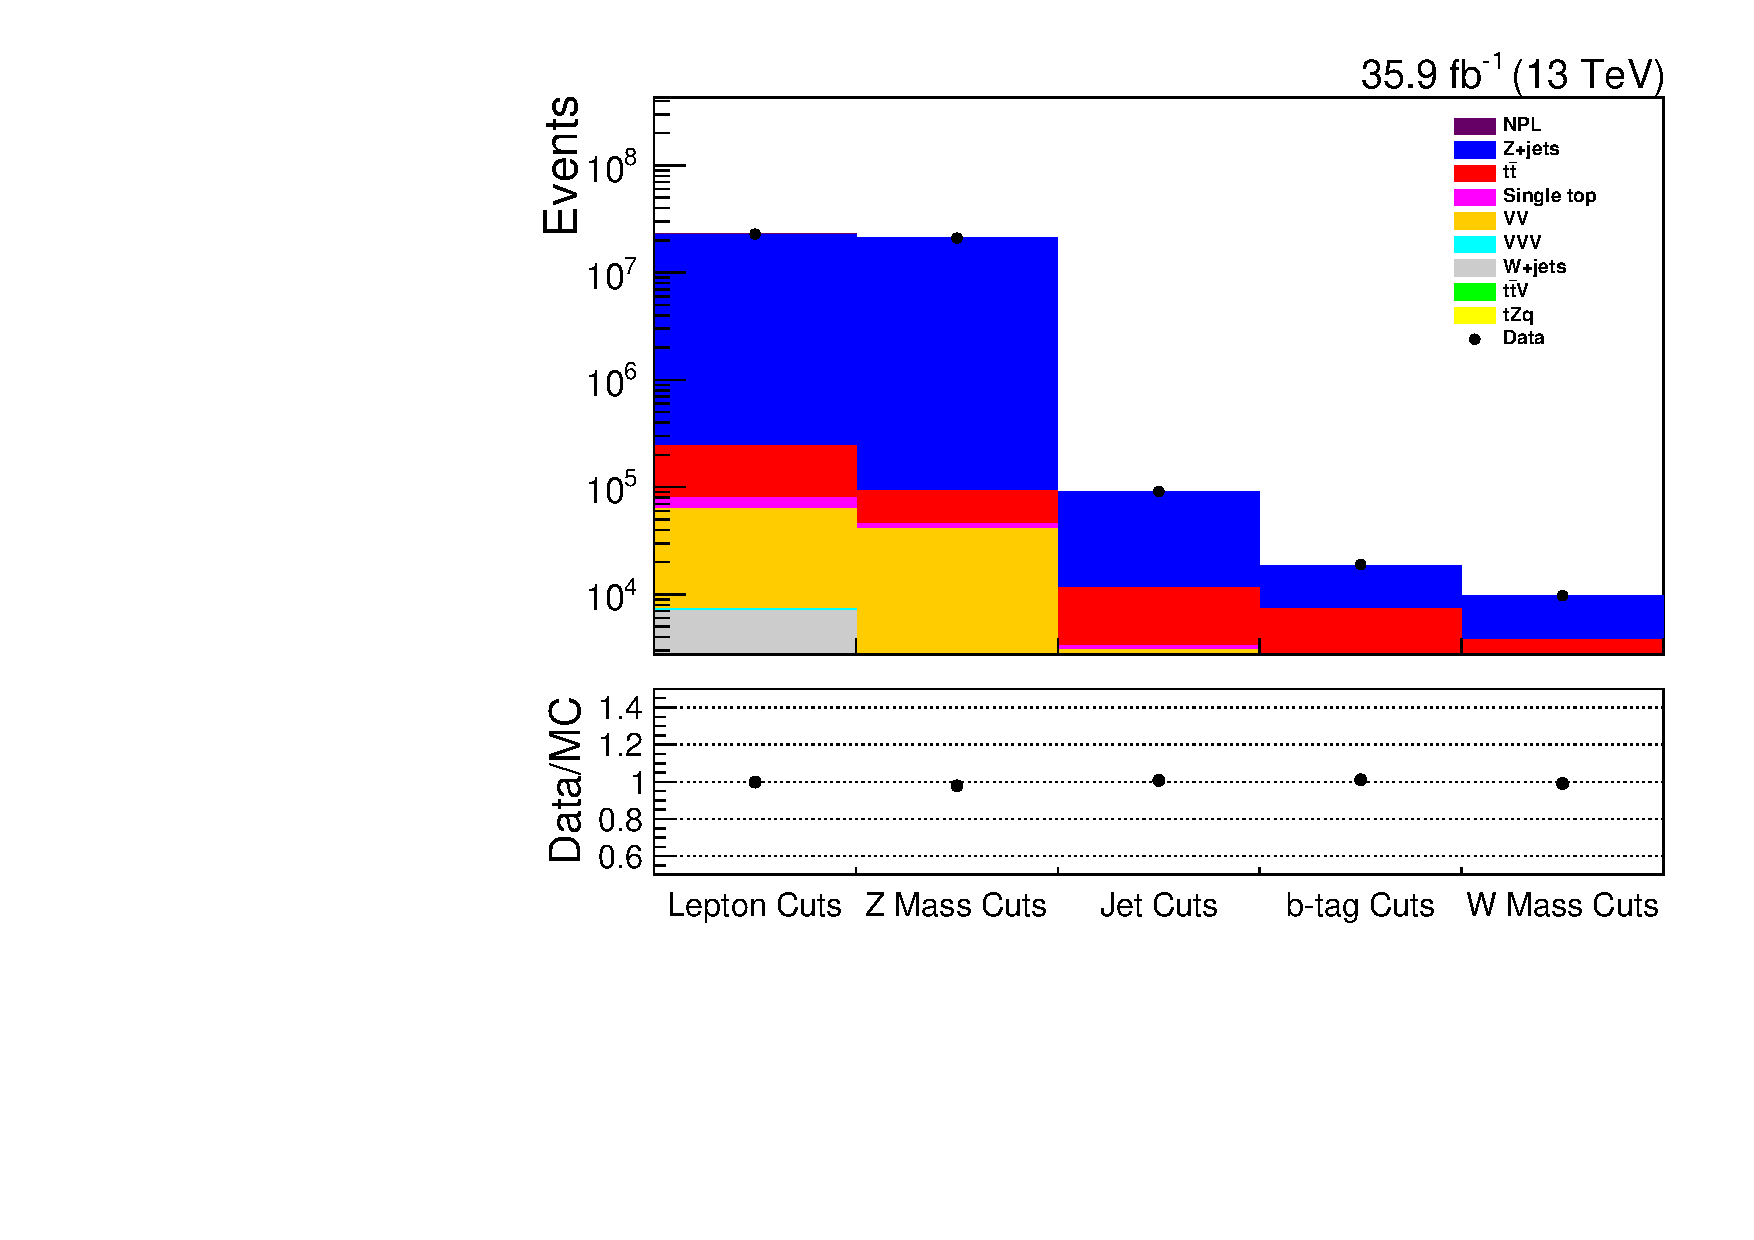
\includegraphics[width=0.97\textwidth]{figs/background-estimation/plots/unblinded/prompt_mumu_ttbarInc/cutFlow_log.pdf}
\caption{
The overall event yield for data and simulation at each stage of applying the signal region selection criteria and simulation corrections.
}
\label{fig:SR_cutFlow}
\end{figure}

\begin{figure}[h]
\centering
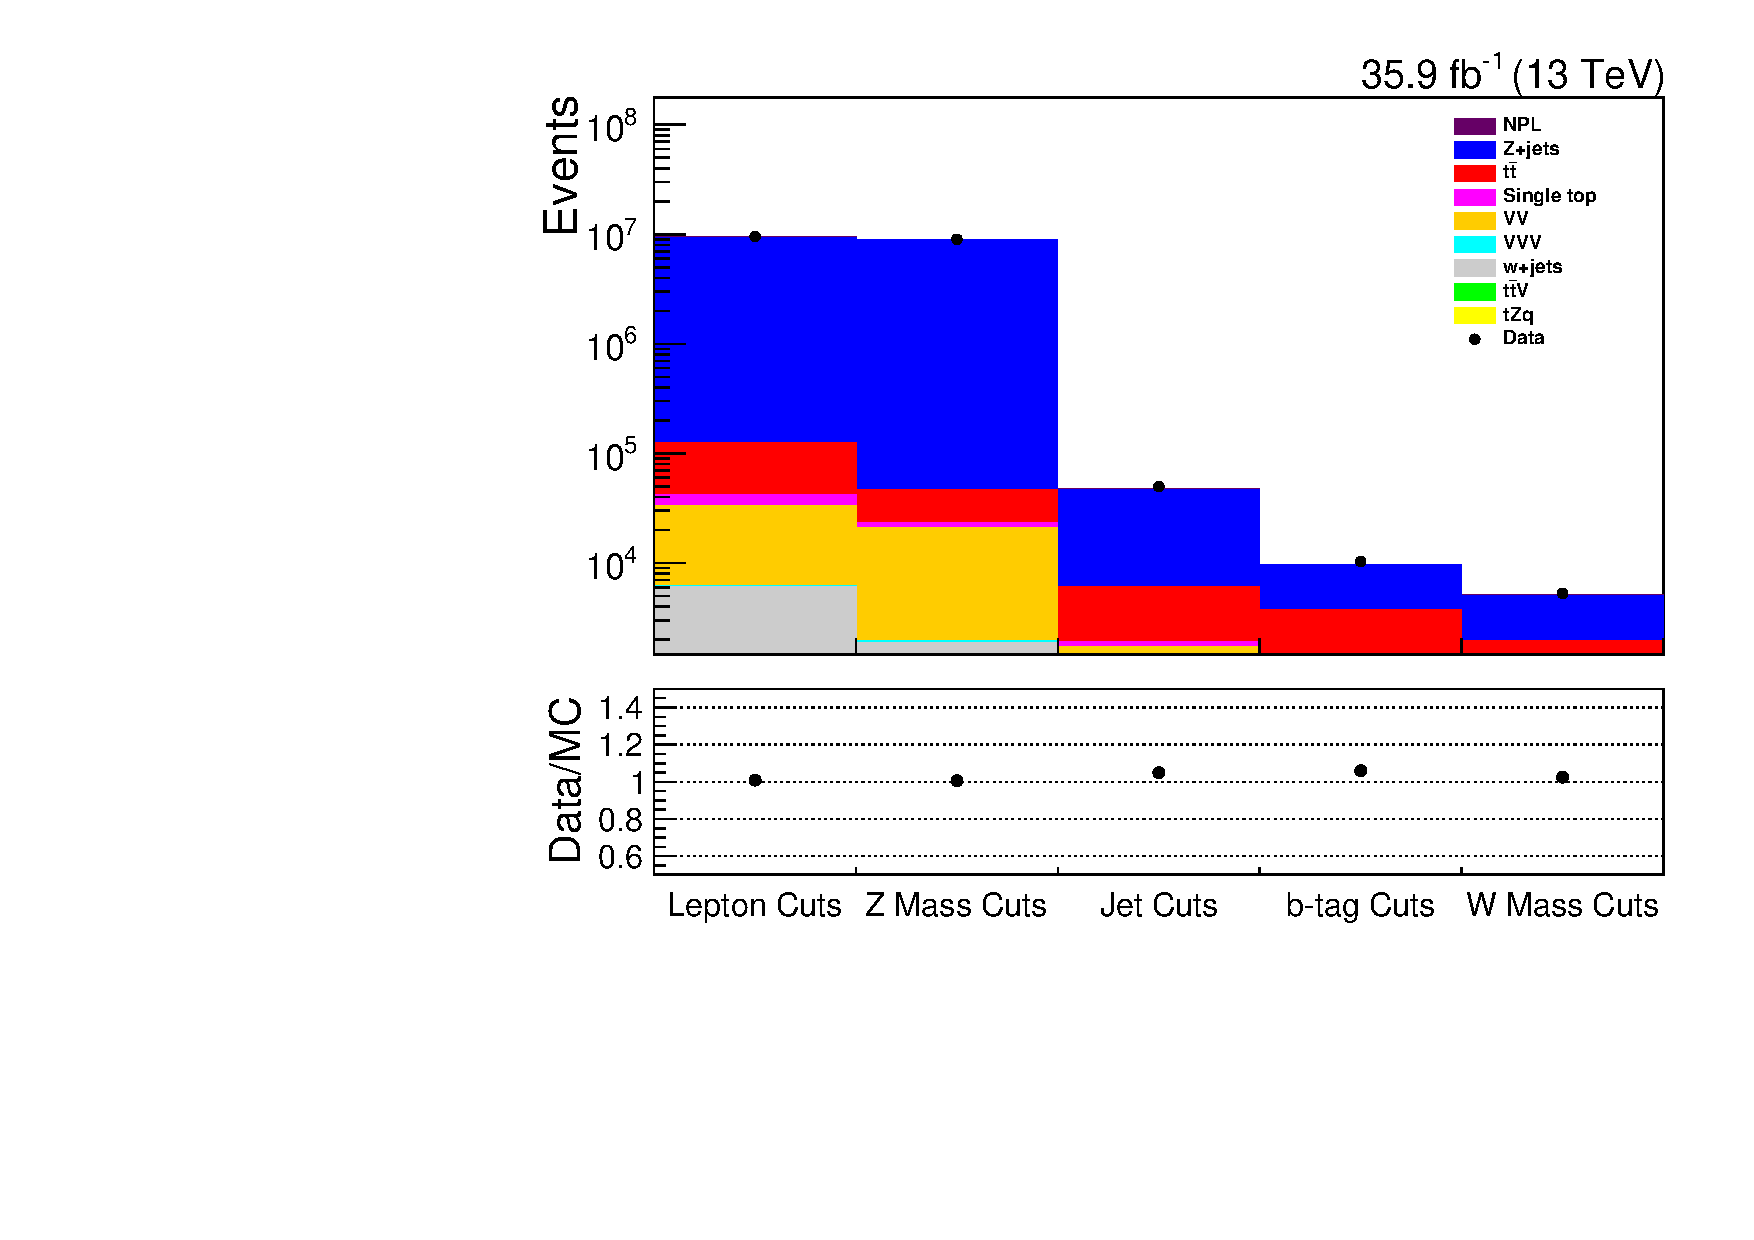
\includegraphics[width=0.47\textwidth]{figs/background-estimation/plots/unblinded/prompt_ee_ttbarInc/cutFlow_log.pdf}
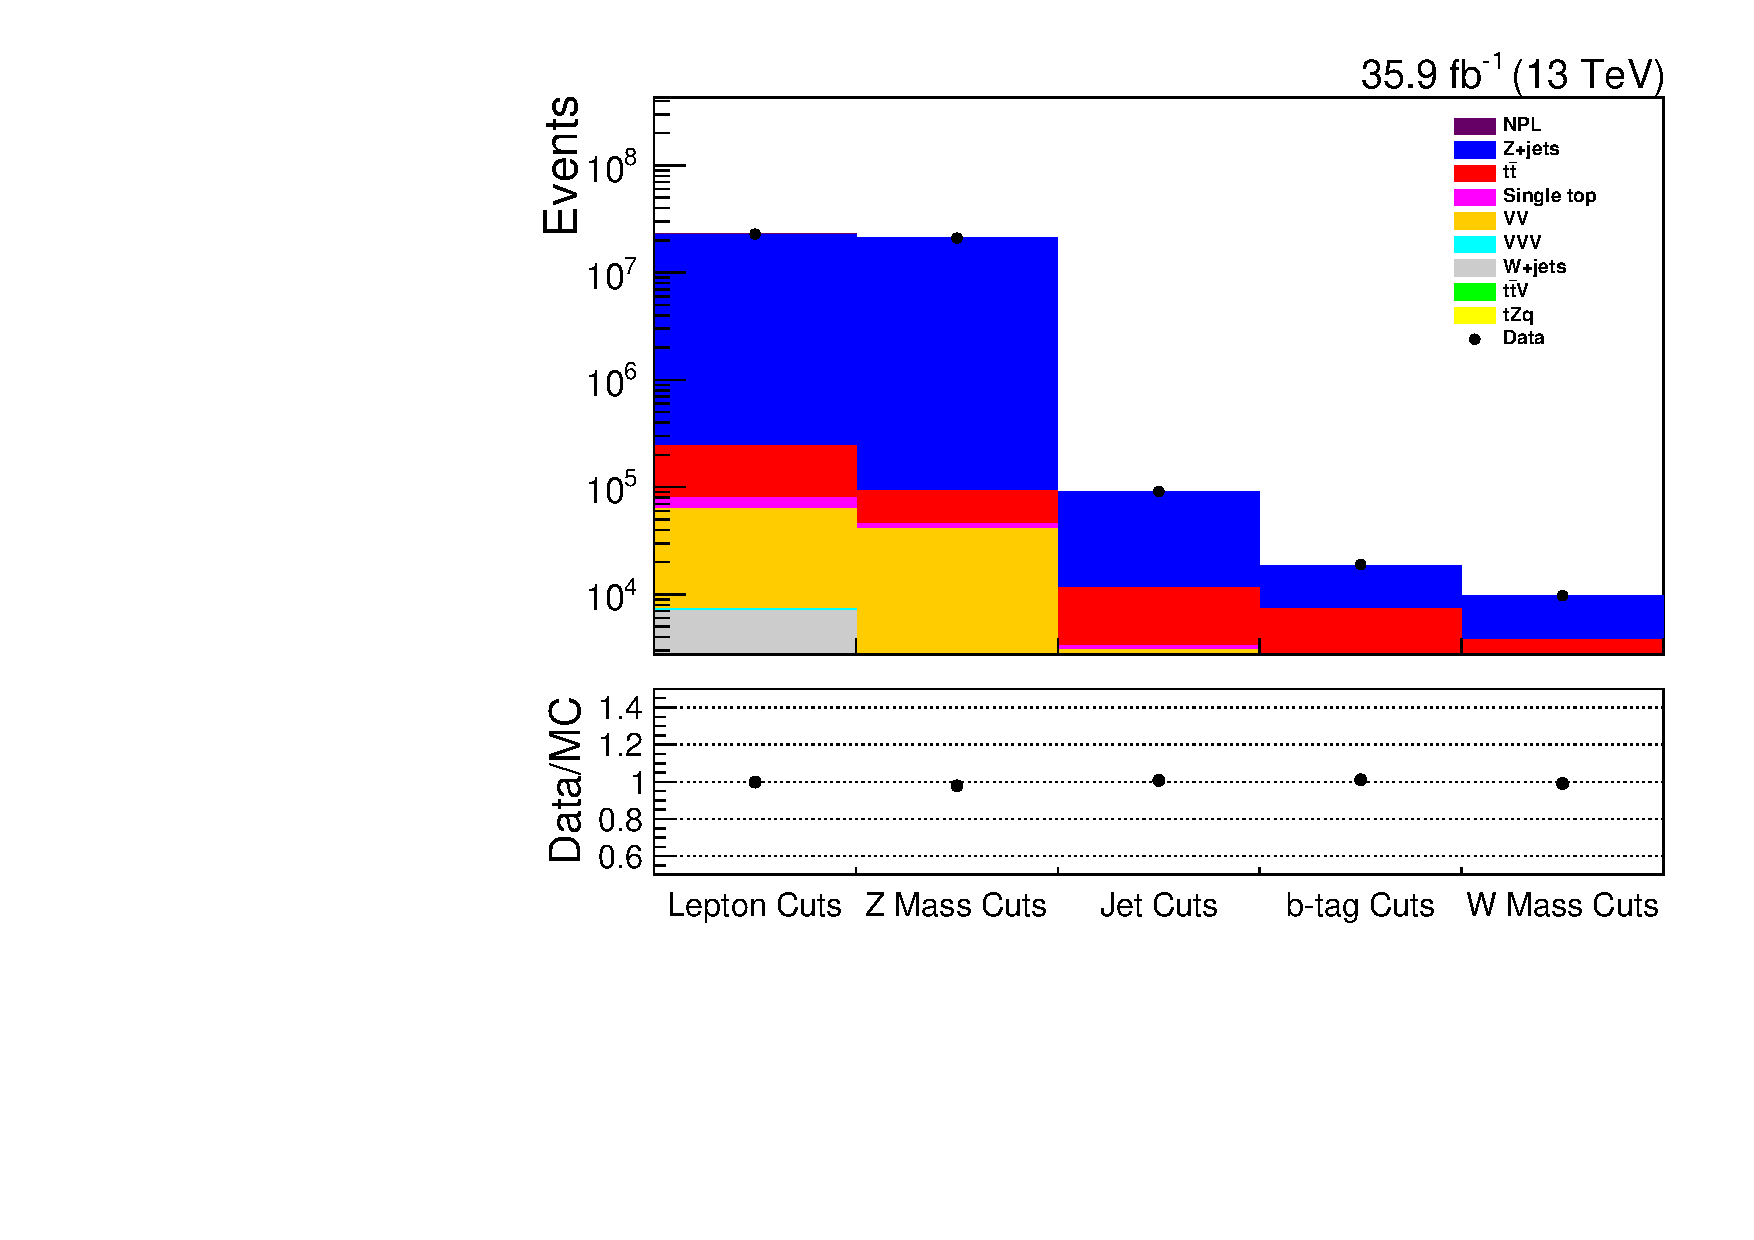
\includegraphics[width=0.47\textwidth]{figs/background-estimation/plots/unblinded/prompt_mumu_ttbarInc/cutFlow_log.pdf}
\\
\caption{
The overall event yield for data and simulation at each stage of applying the signal region selection criteria and simulation corrections for the $ee$ channel (left) and the $\mu\mu$ channel (right).
}
\label{fig:SR_lep1Pt}
\end{figure}

\begin{figure}[h]
\centering
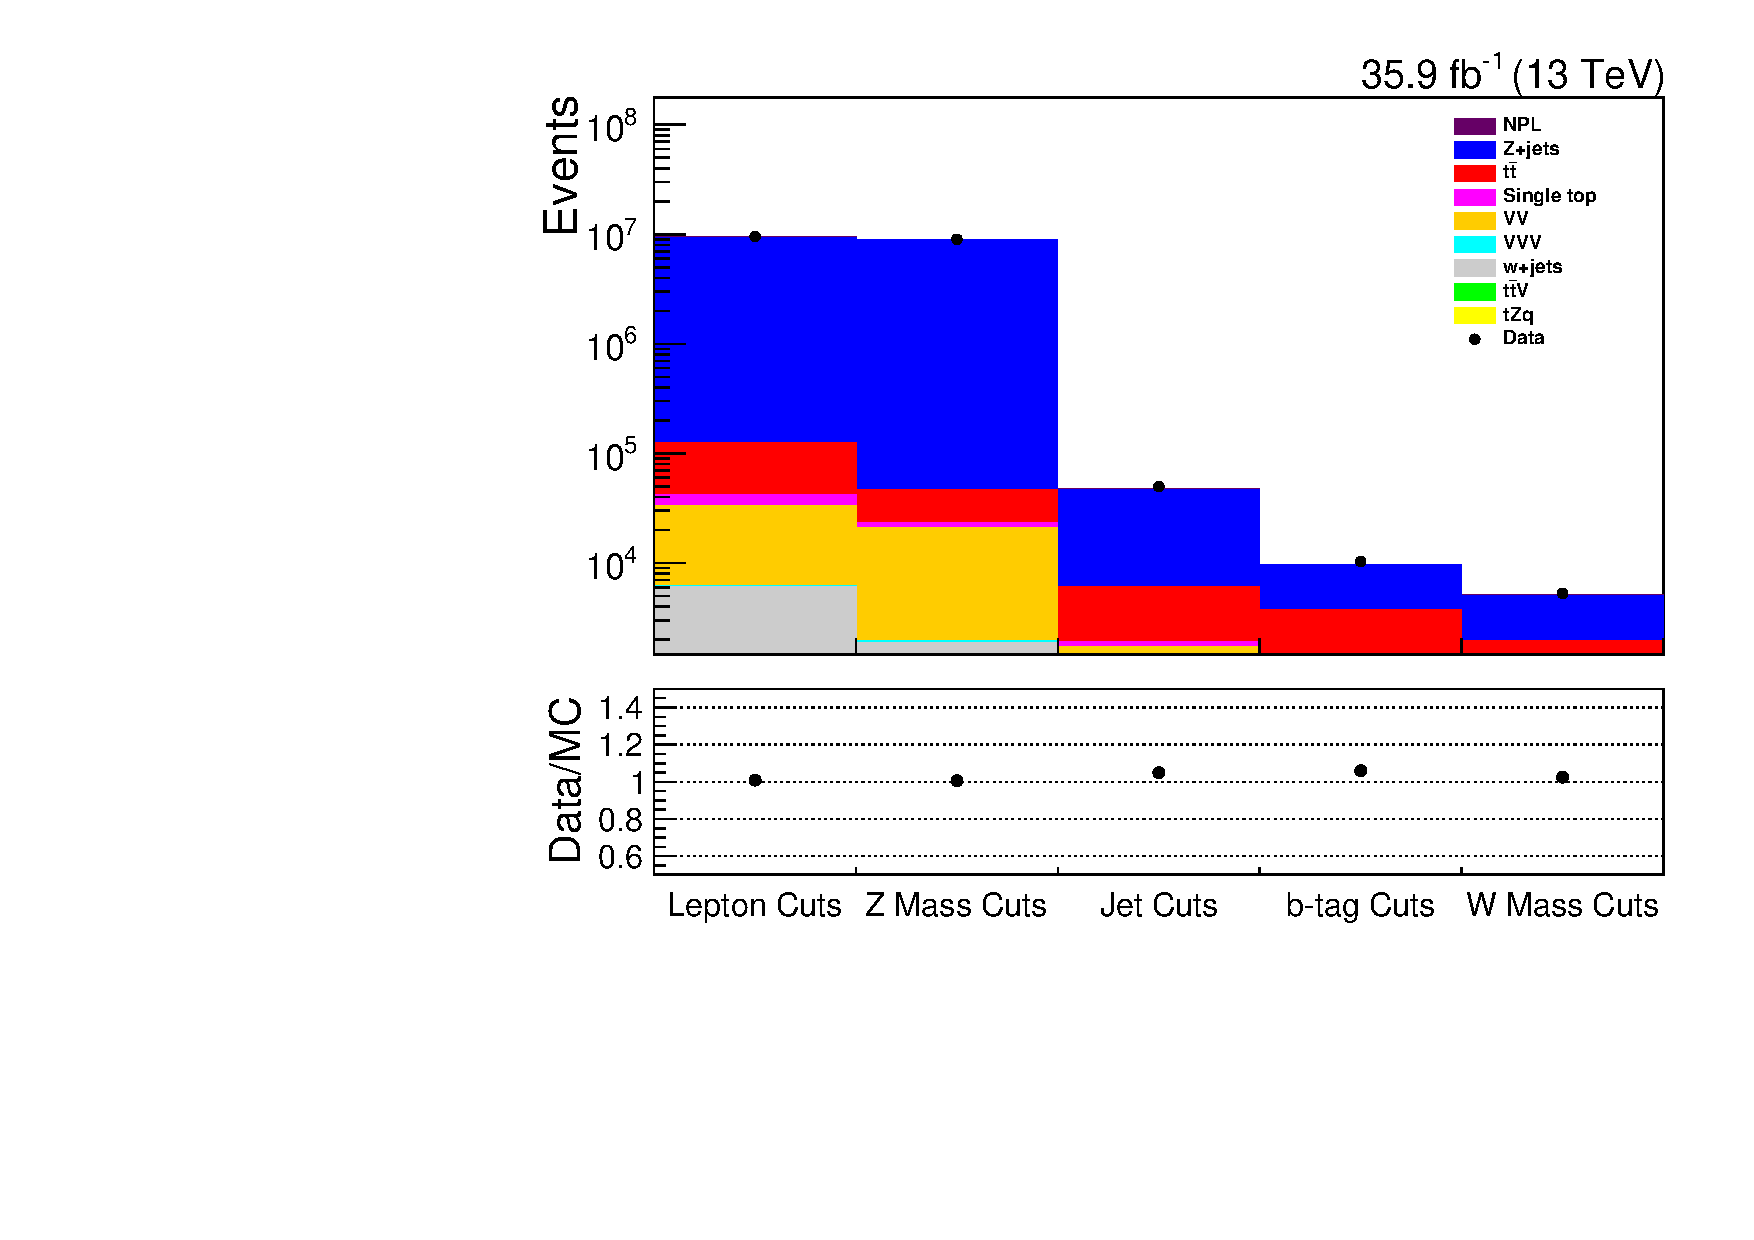
\includegraphics[width=0.47\textwidth]{figs/background-estimation/plots/unblinded/prompt_ee_ttbarInc/cutFlow_log.pdf}
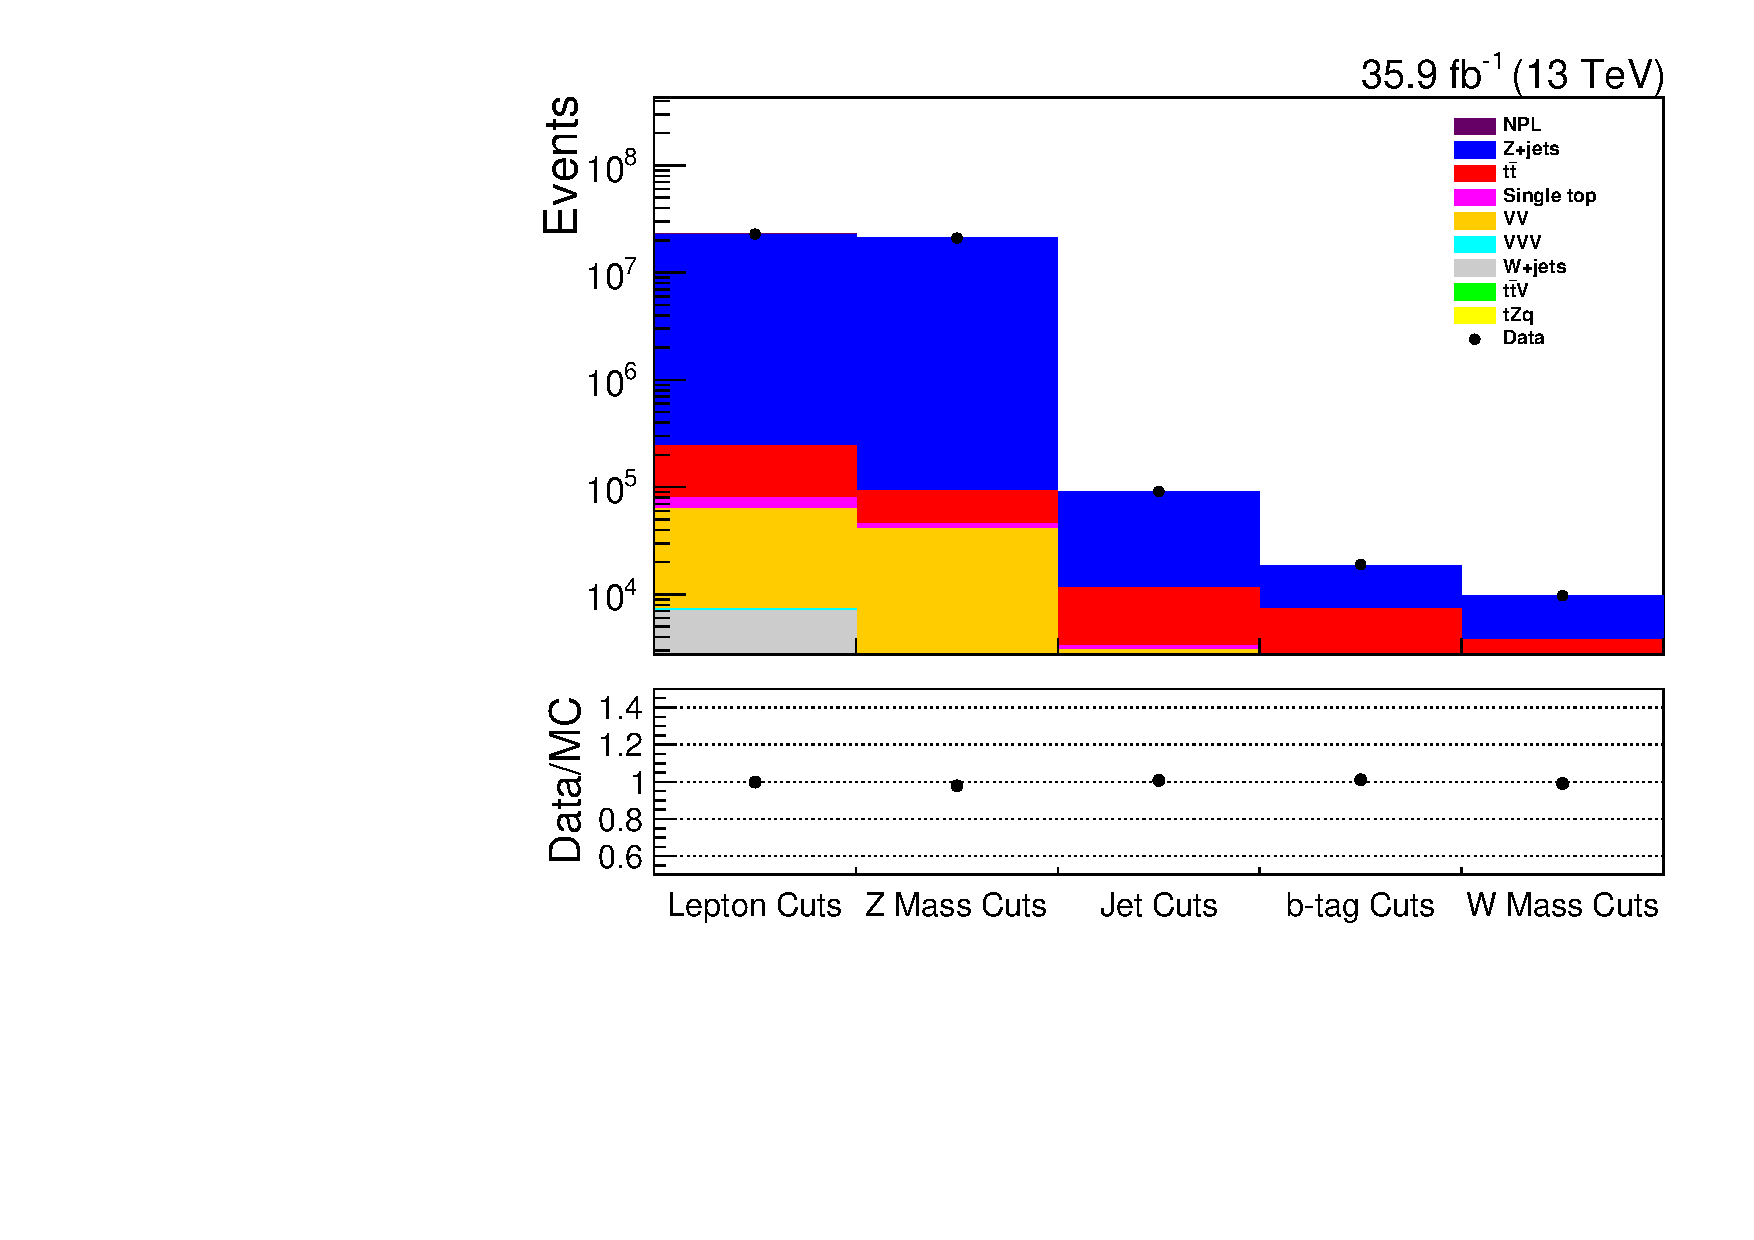
\includegraphics[width=0.47\textwidth]{figs/background-estimation/plots/unblinded/prompt_mumu_ttbarInc/cutFlow_log.pdf}
\caption{
The overall event yield for data and simulation at each stage of applying the signal region selection criteria and simulation corrections for the $ee$ channel (left) and the $\mu\mu$ channel (right).
}
\label{fig:SR_lep2Pt}
\end{figure}

\begin{figure}[h]
\centering
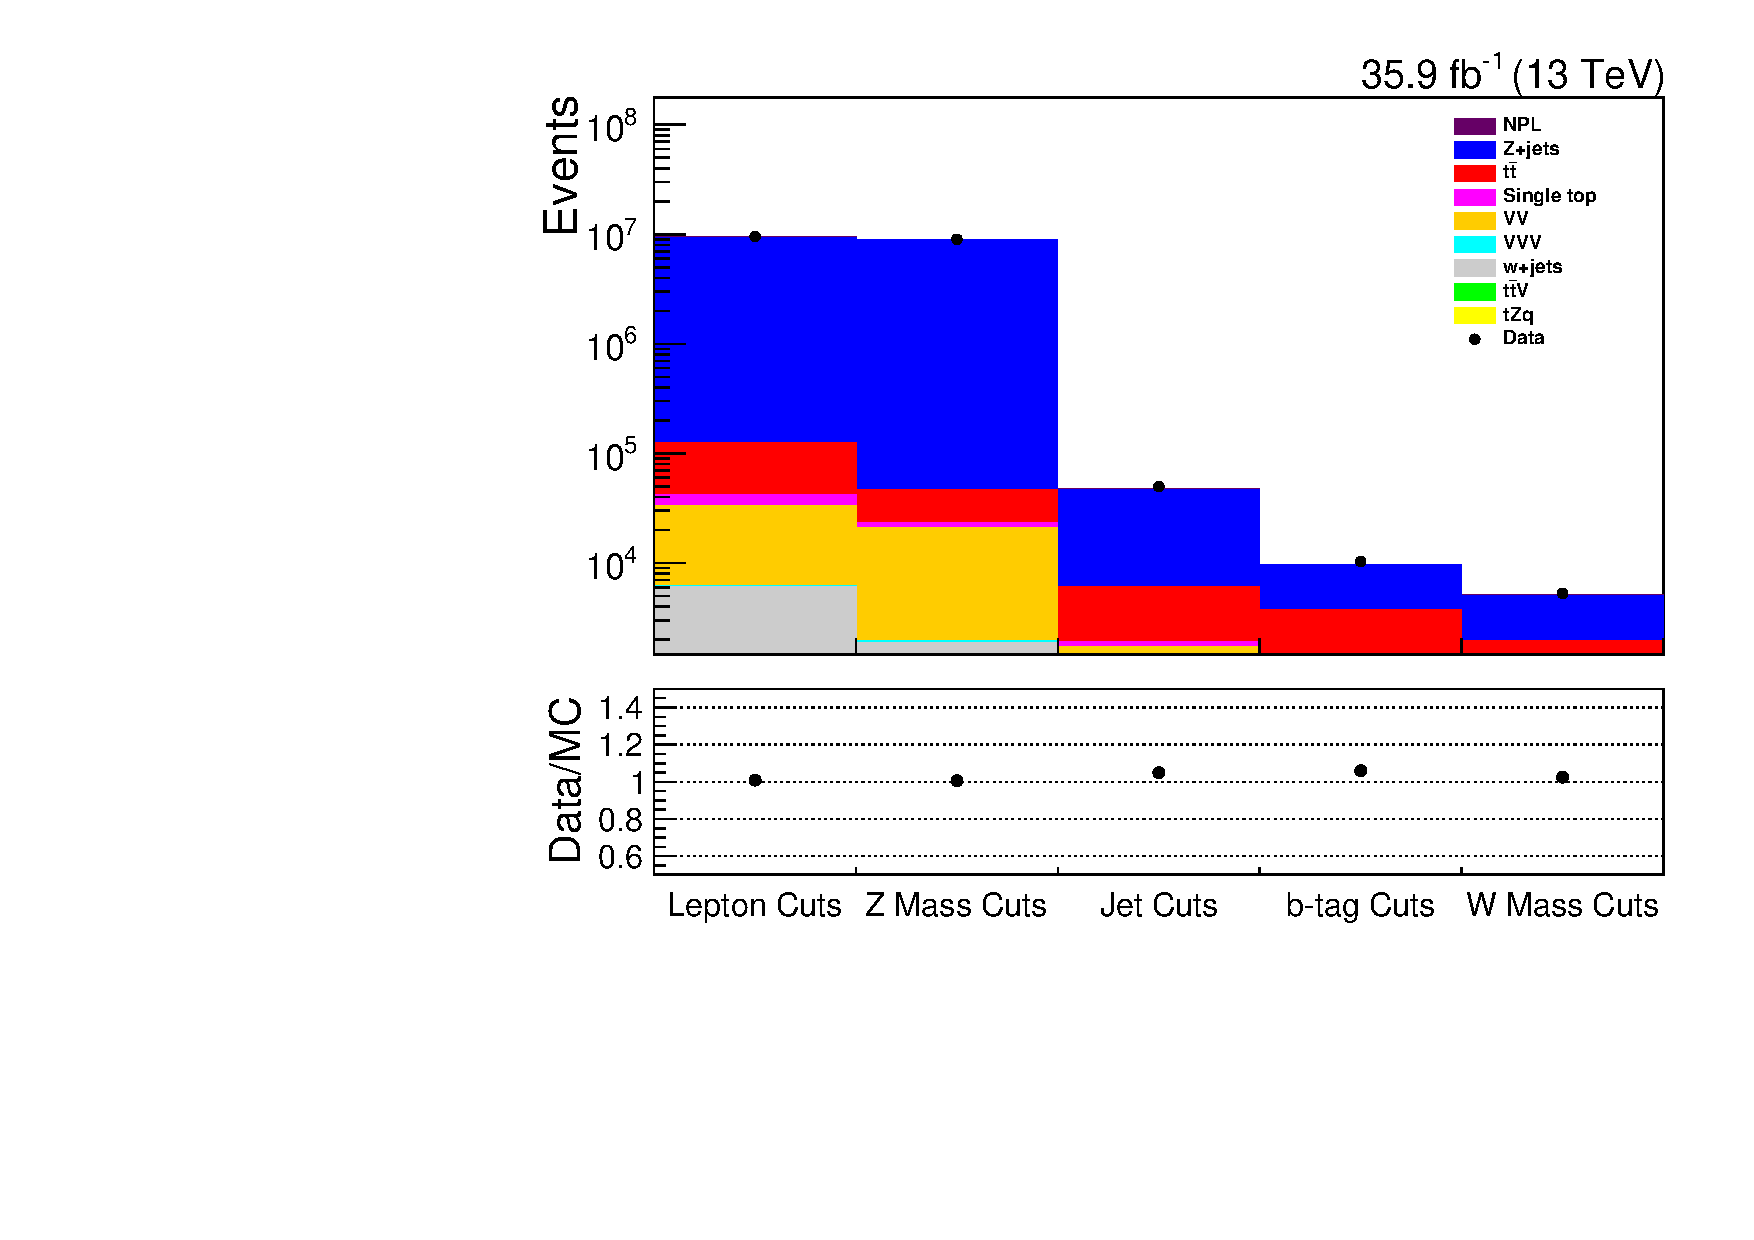
\includegraphics[width=0.47\textwidth]{figs/background-estimation/plots/unblinded/prompt_ee_ttbarInc/cutFlow_log.pdf}
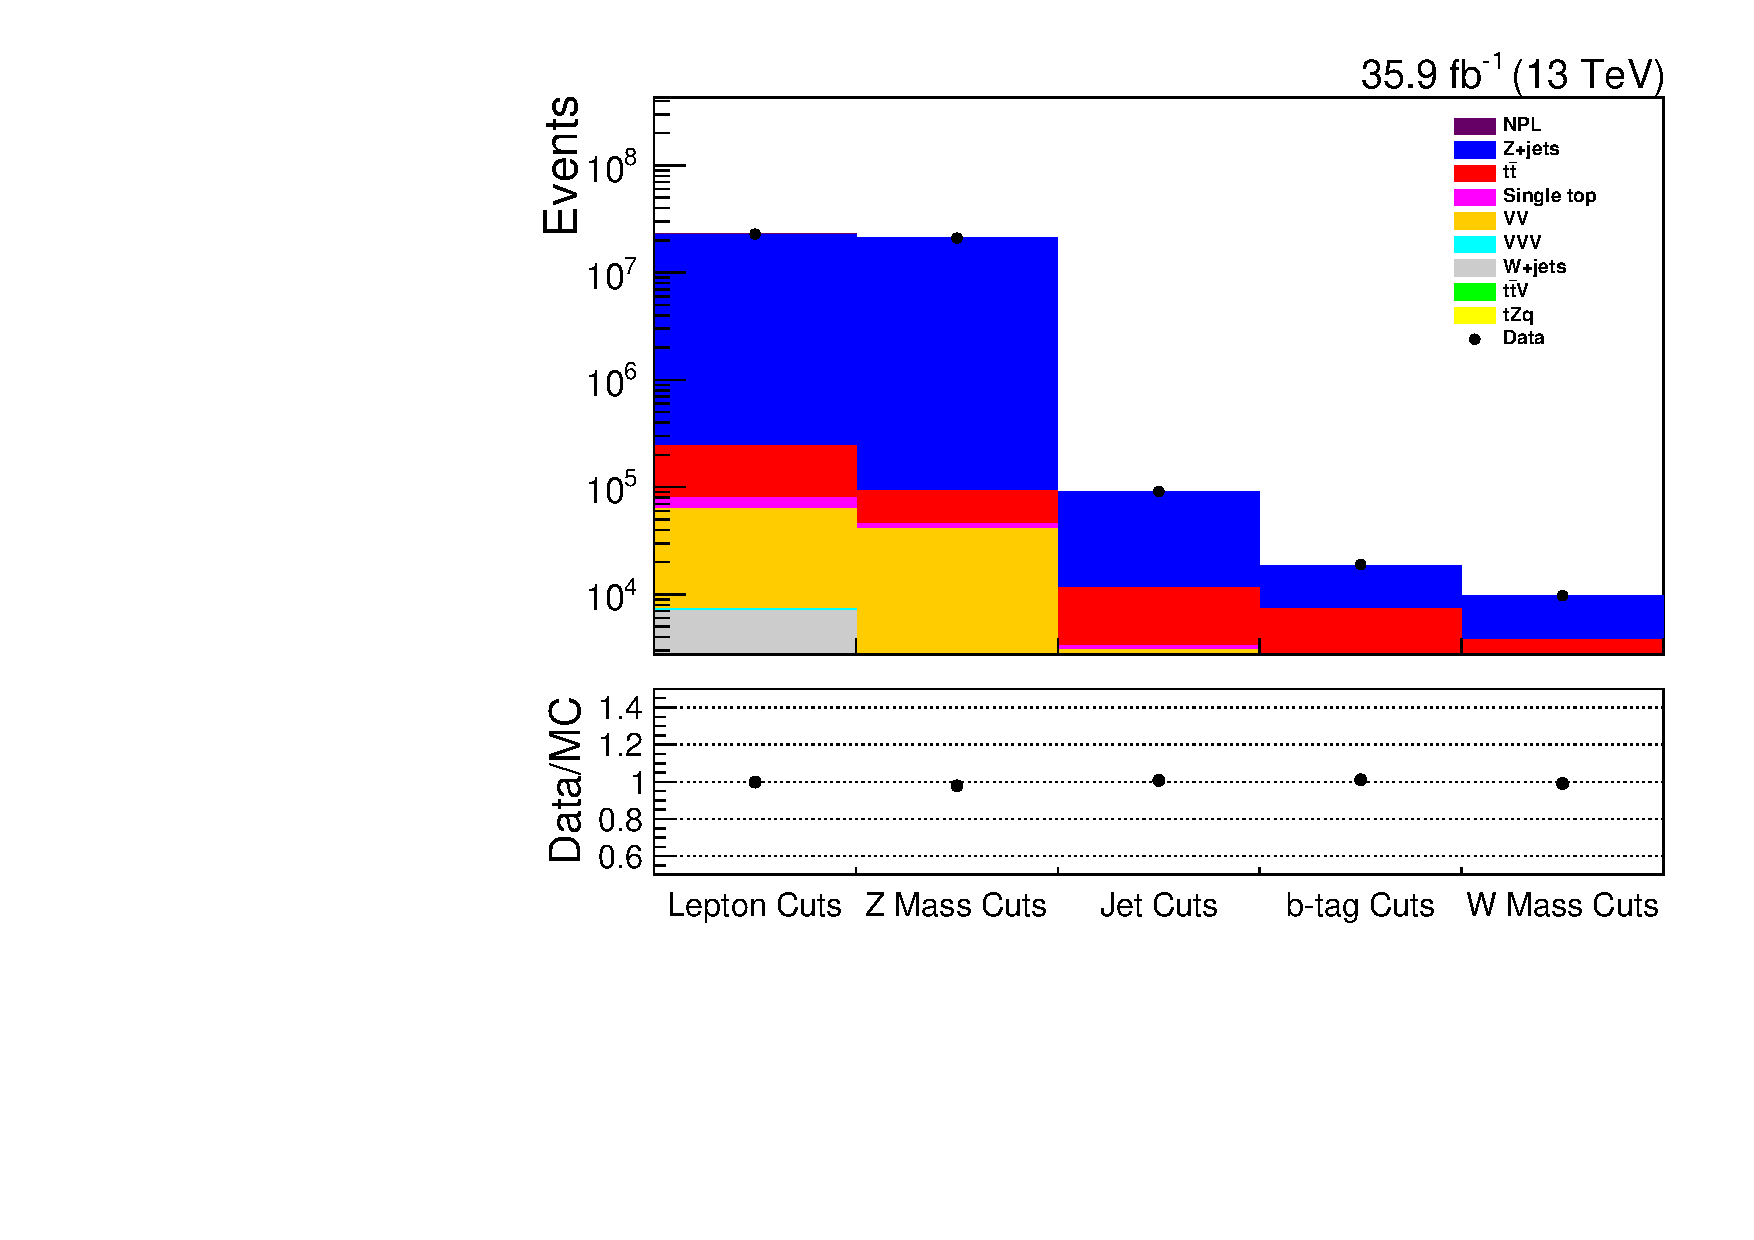
\includegraphics[width=0.47\textwidth]{figs/background-estimation/plots/unblinded/prompt_mumu_ttbarInc/cutFlow_log.pdf}
\caption{
The overall event yield for data and simulation at each stage of applying the signal region selection criteria and simulation corrections for the $ee$ channel (left) and the $\mu\mu$ channel (right).
}
\label{fig:SR_lep1Eta}
\end{figure}

\begin{figure}[h]
\centering
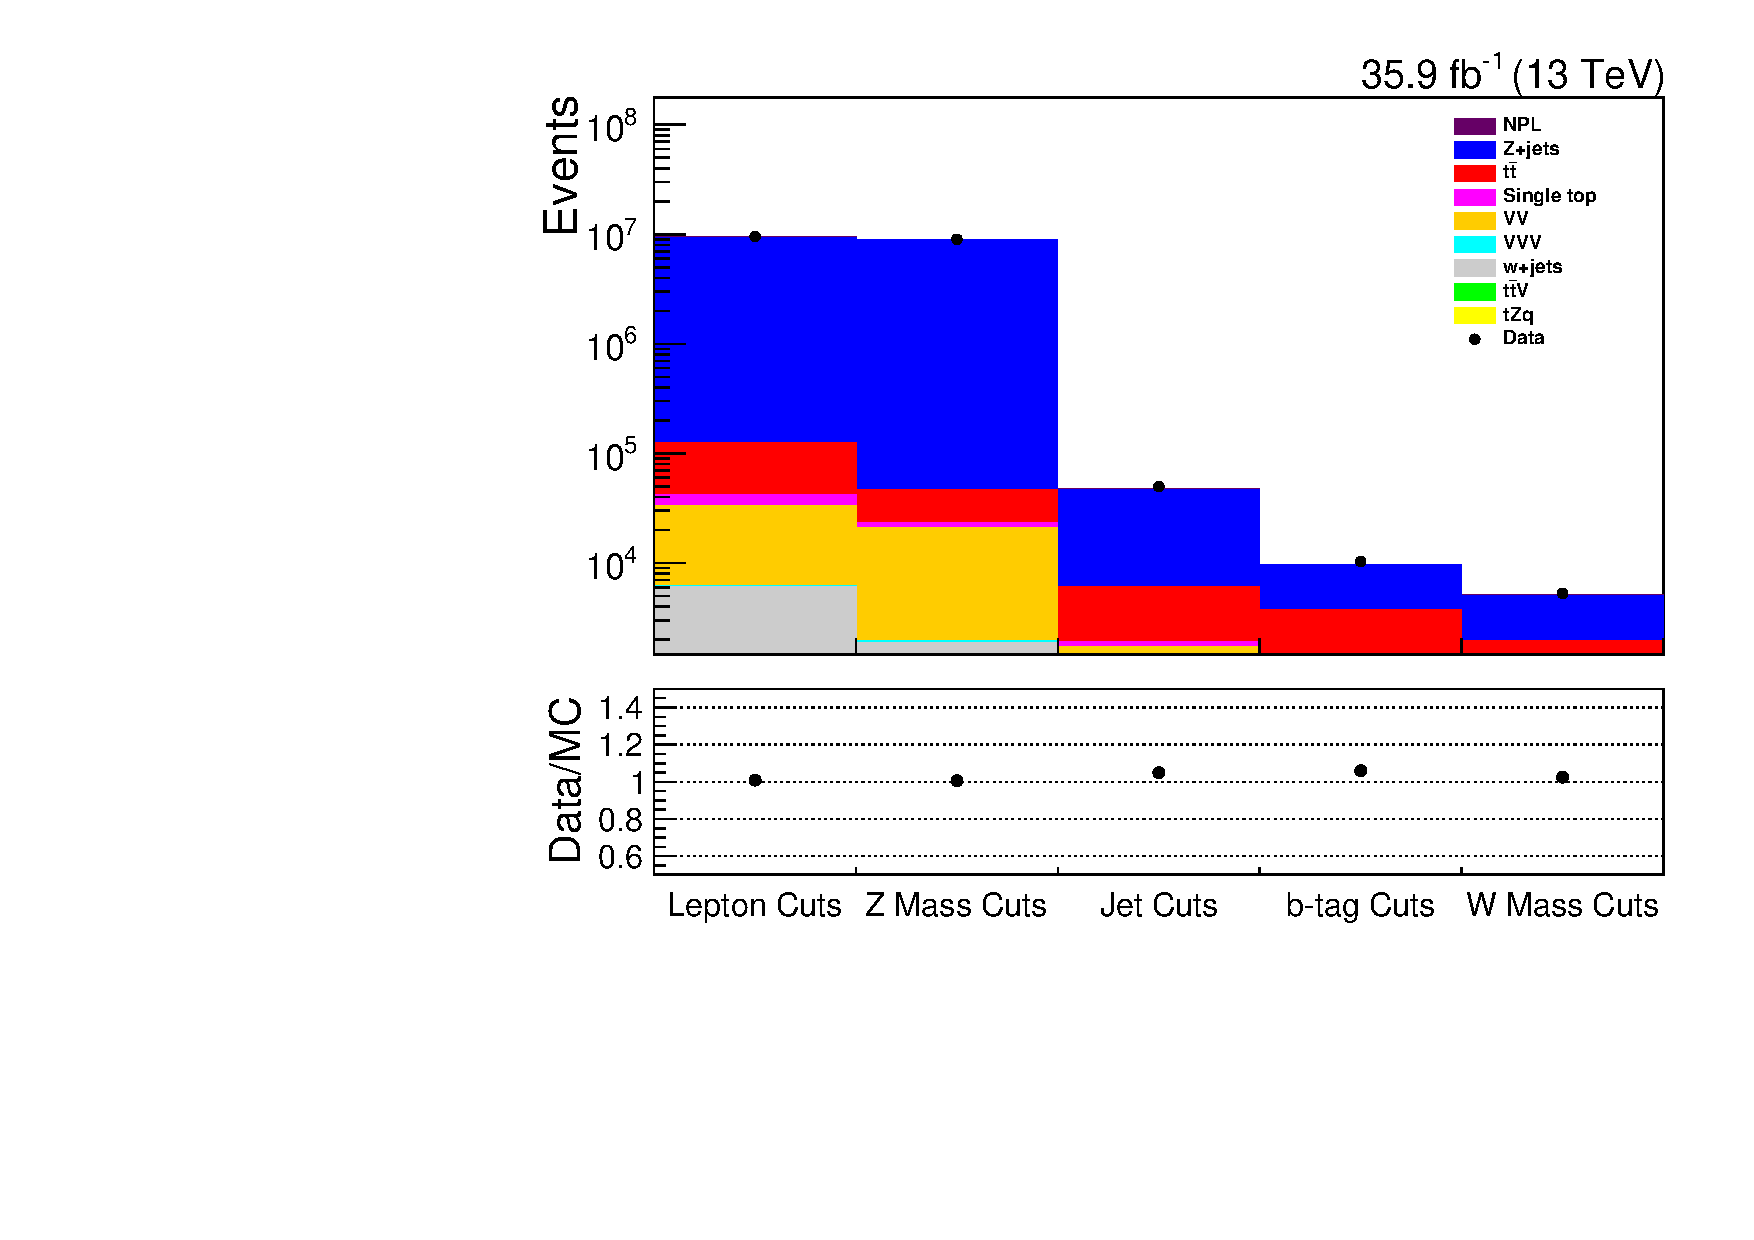
\includegraphics[width=0.47\textwidth]{figs/background-estimation/plots/unblinded/prompt_ee_ttbarInc/cutFlow_log.pdf}
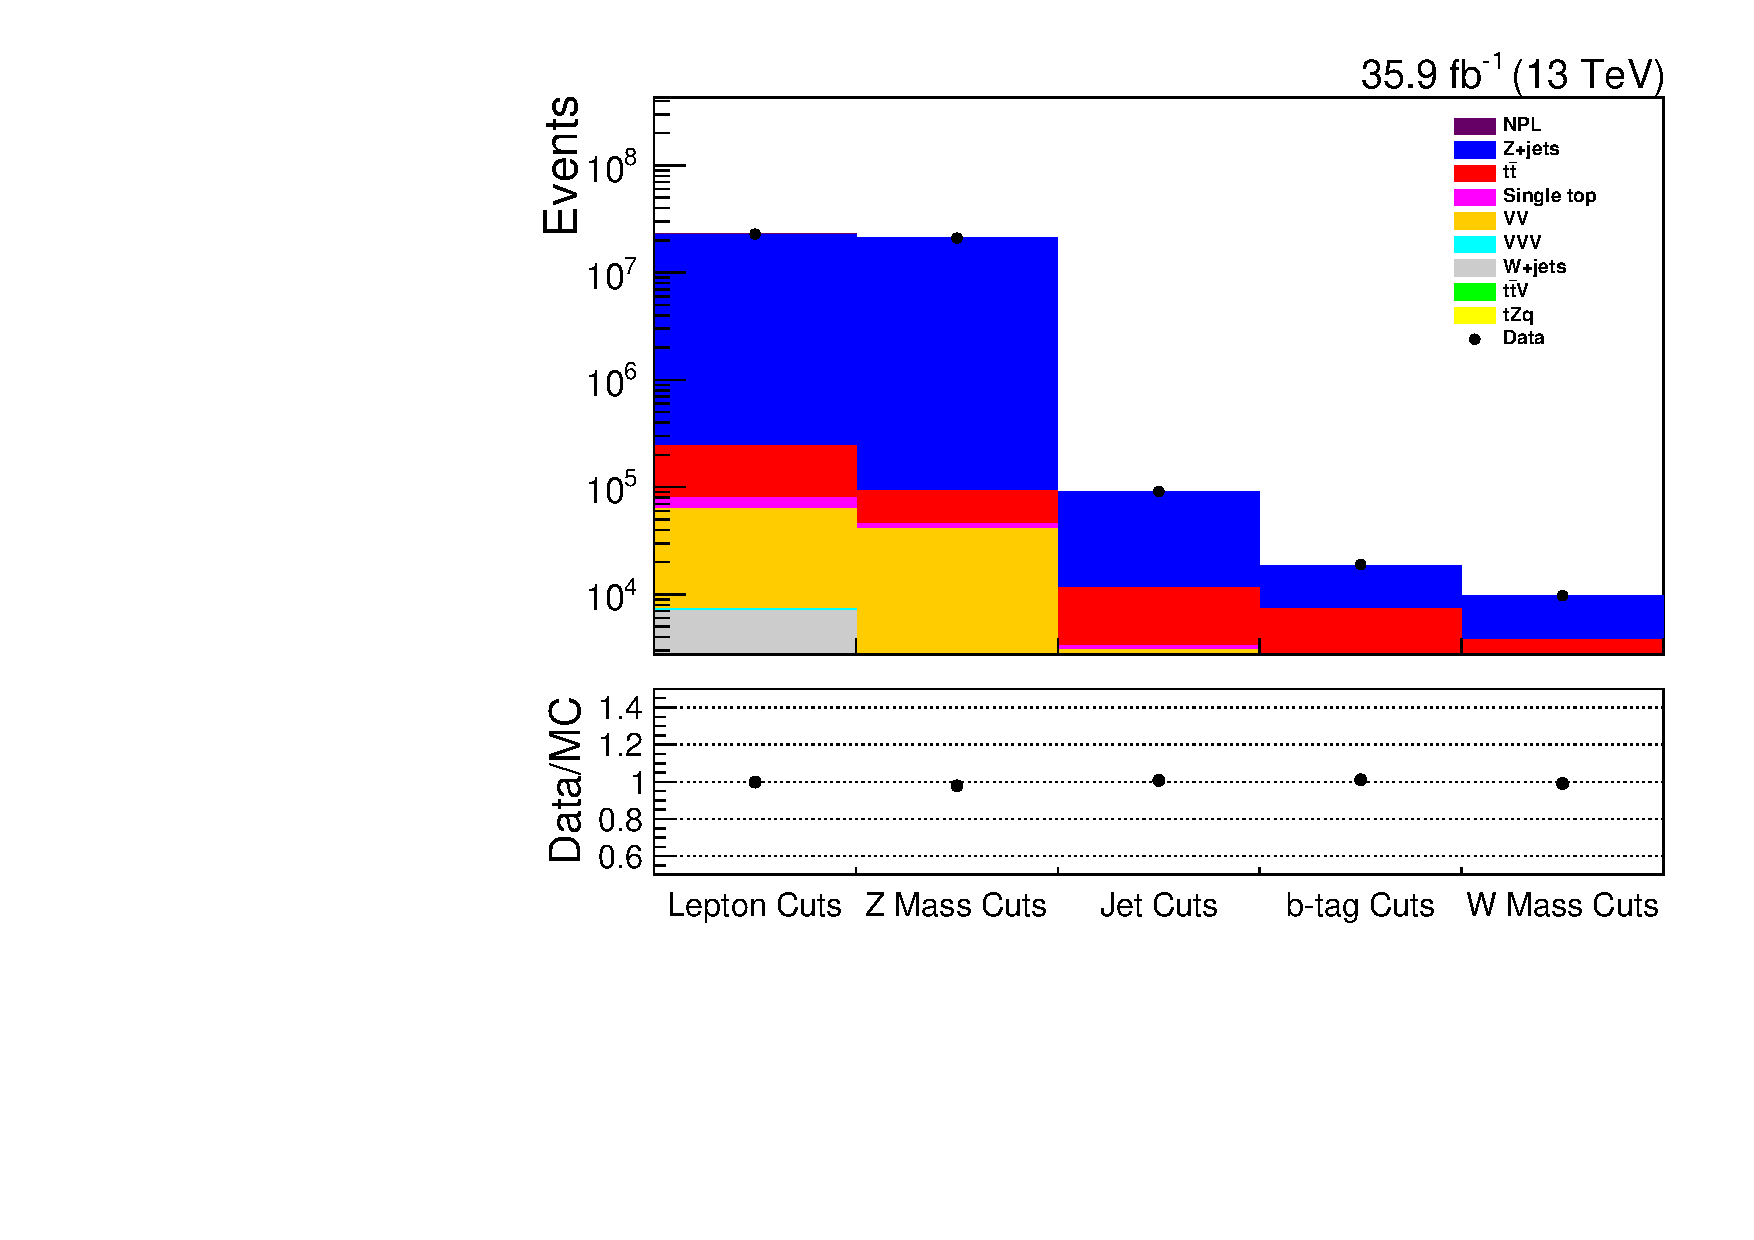
\includegraphics[width=0.47\textwidth]{figs/background-estimation/plots/unblinded/prompt_mumu_ttbarInc/cutFlow_log.pdf}
\caption{
The overall event yield for data and simulation at each stage of applying the signal region selection criteria and simulation corrections for the $ee$ channel (left) and the $\mu\mu$ channel (right).
}
\label{fig:SR_lep2Eta}
\end{figure}

\section{Z+jets Control Region}\label{appSec:signalRegionPlots}

\section{\ttbar Control Region}\label{appSec:signalRegionPlots}

\begin{figure}[h]
\centering
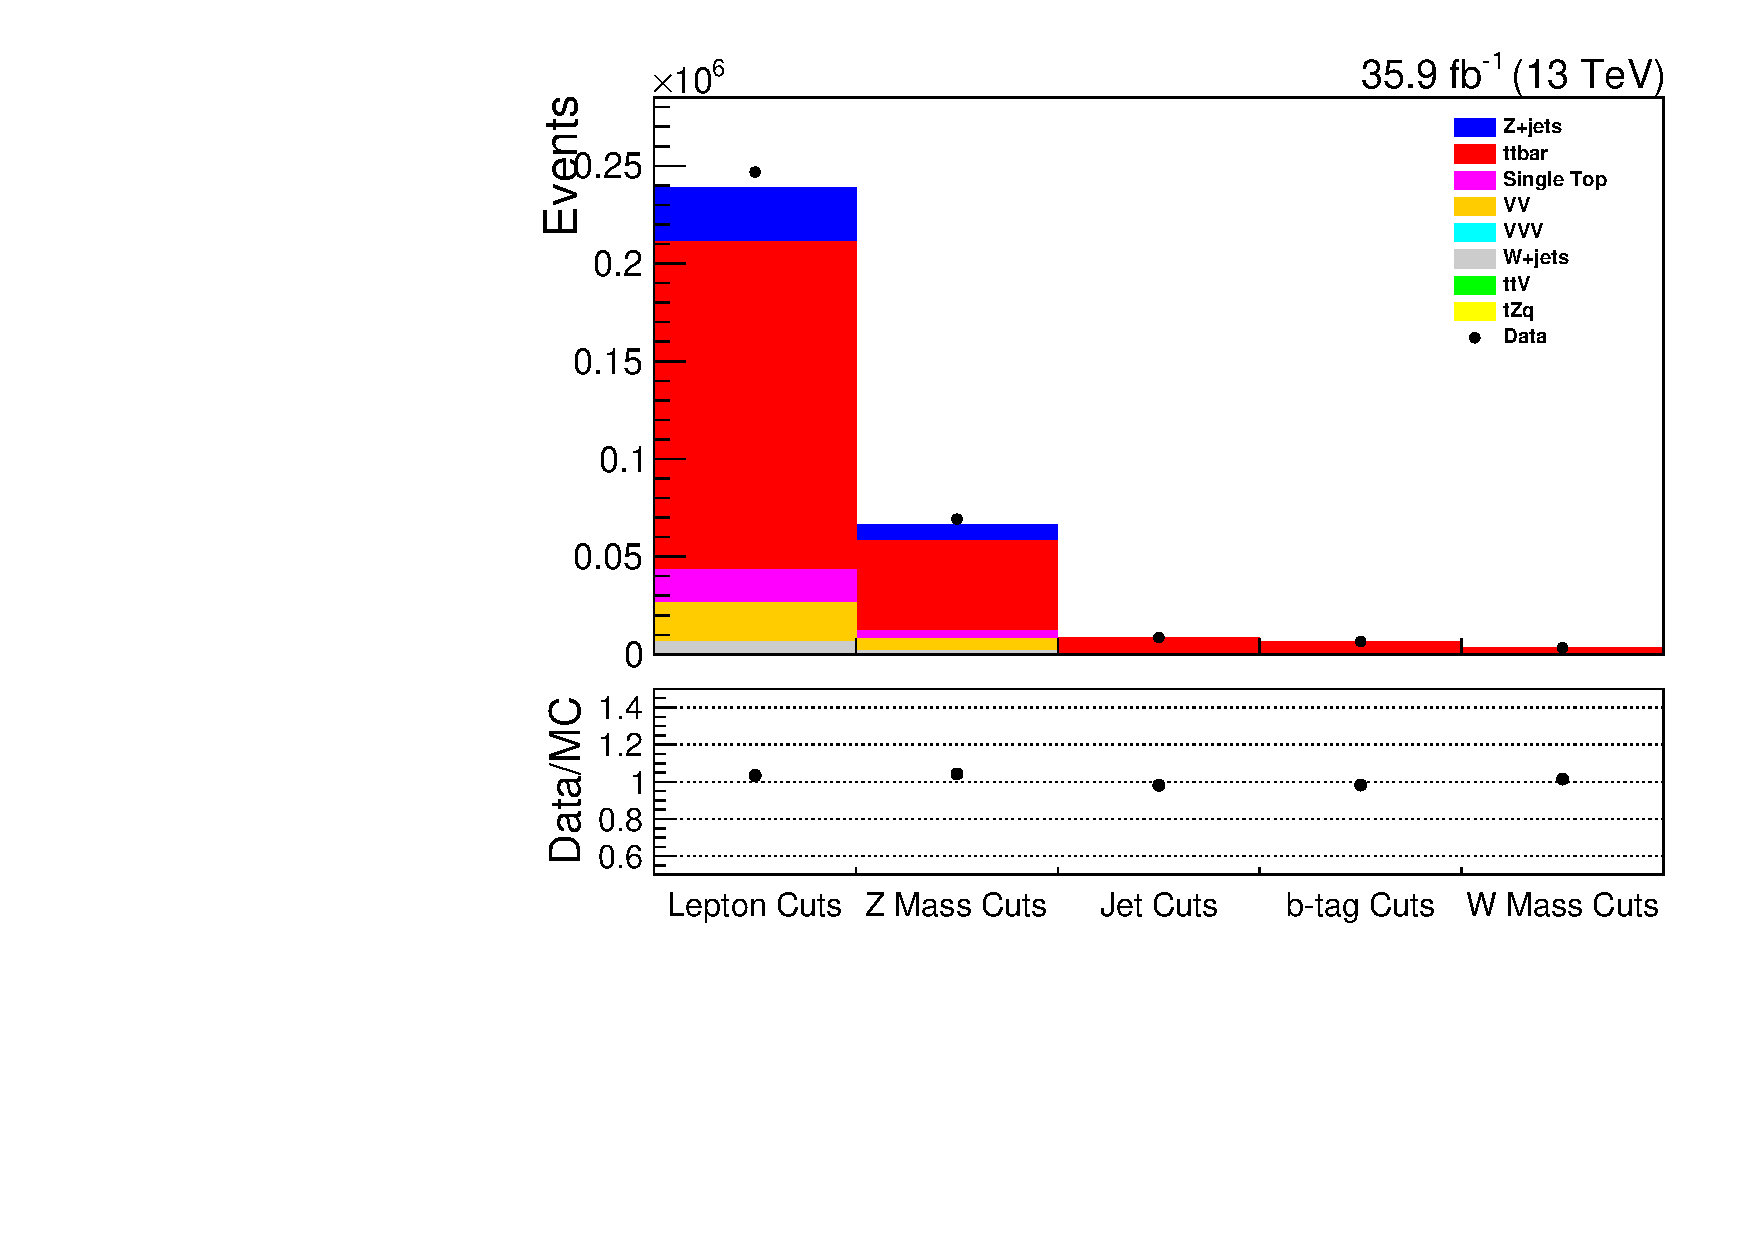
\includegraphics[width=0.97\textwidth]{figs/background-estimation/plots/unblinded/ttbar_control/cutFlow_log.pdf}
\caption{
The overall event yield for data and simulation at each stage of applying the signal region selection criteria and simulation corrections.
}
\label{fig:ttbar_cutFlow}
\end{figure}

\begin{figure}[h]
\centering
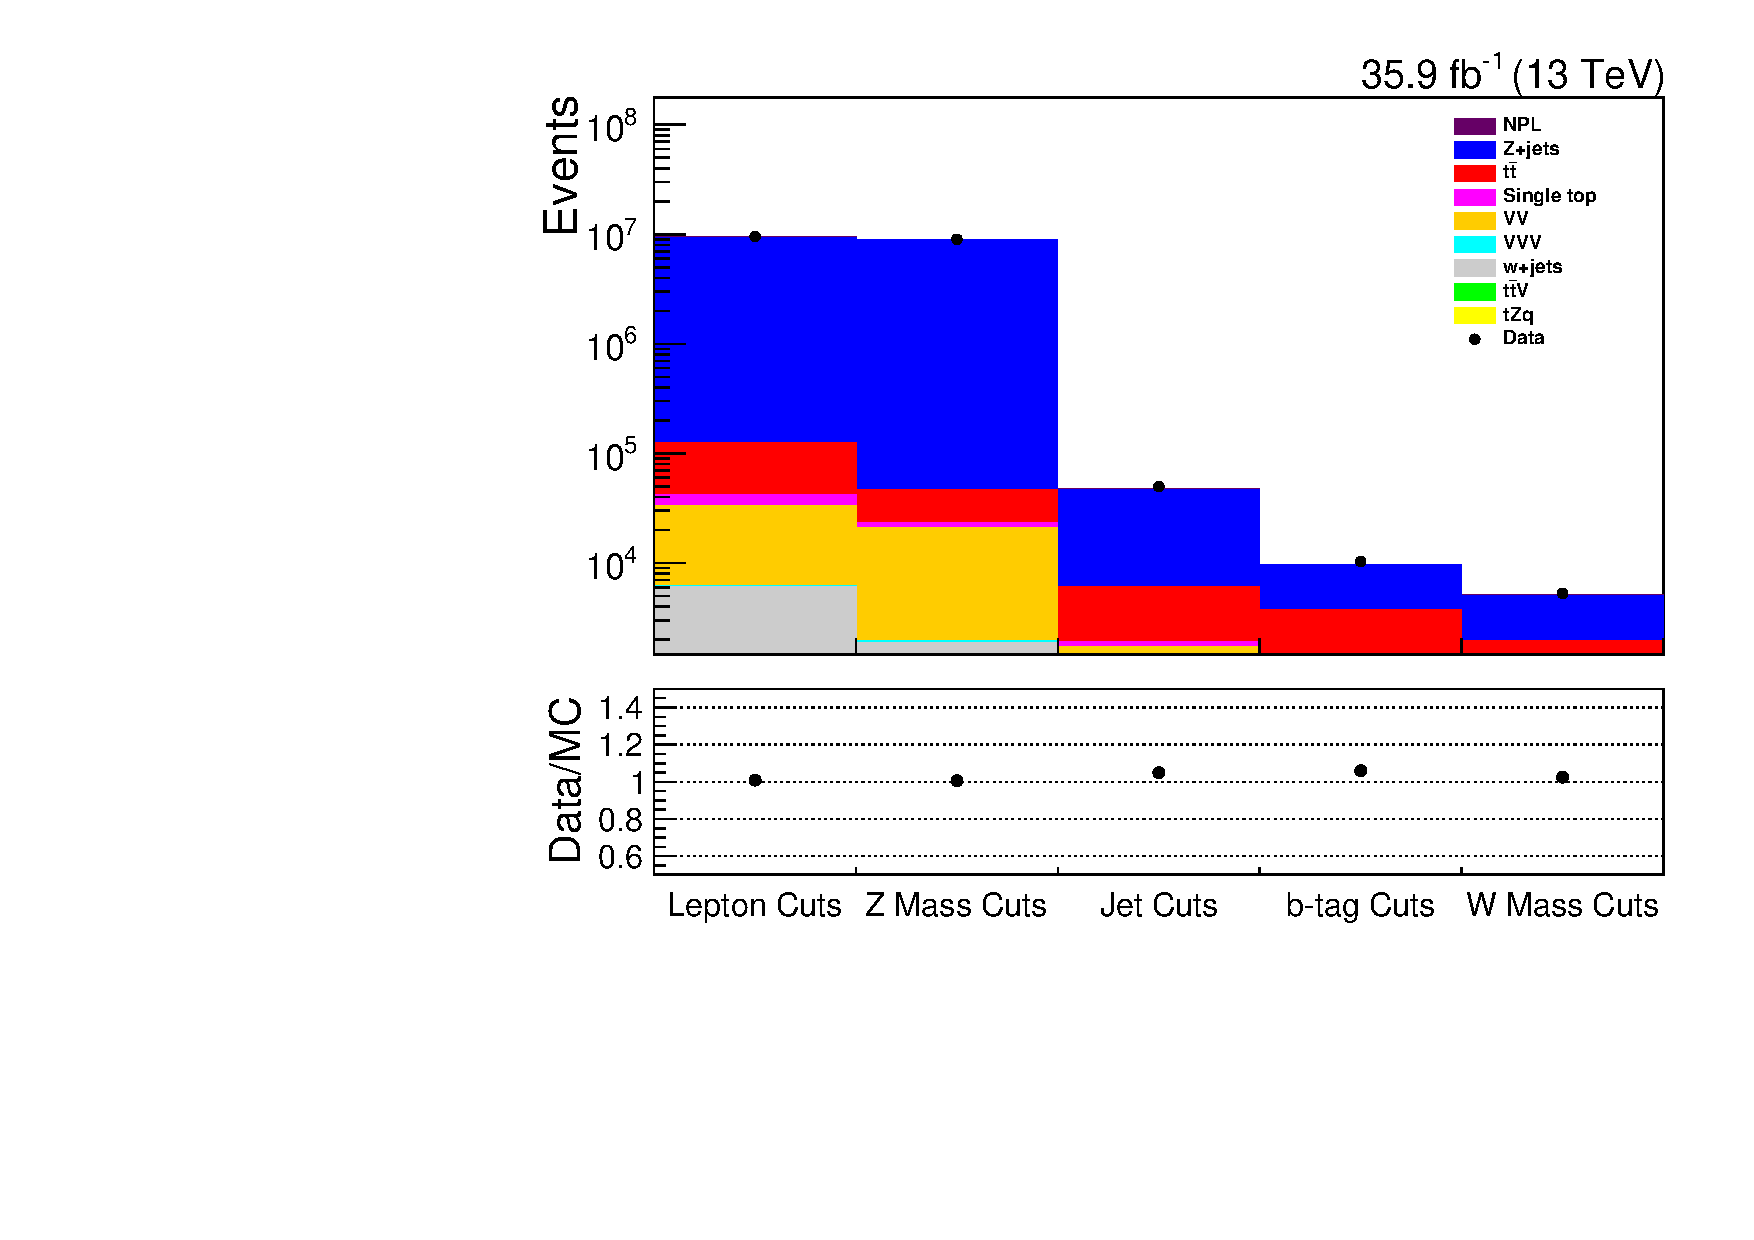
\includegraphics[width=0.47\textwidth]{figs/background-estimation/plots/unblinded/prompt_ee_ttbarInc/cutFlow_log.pdf}
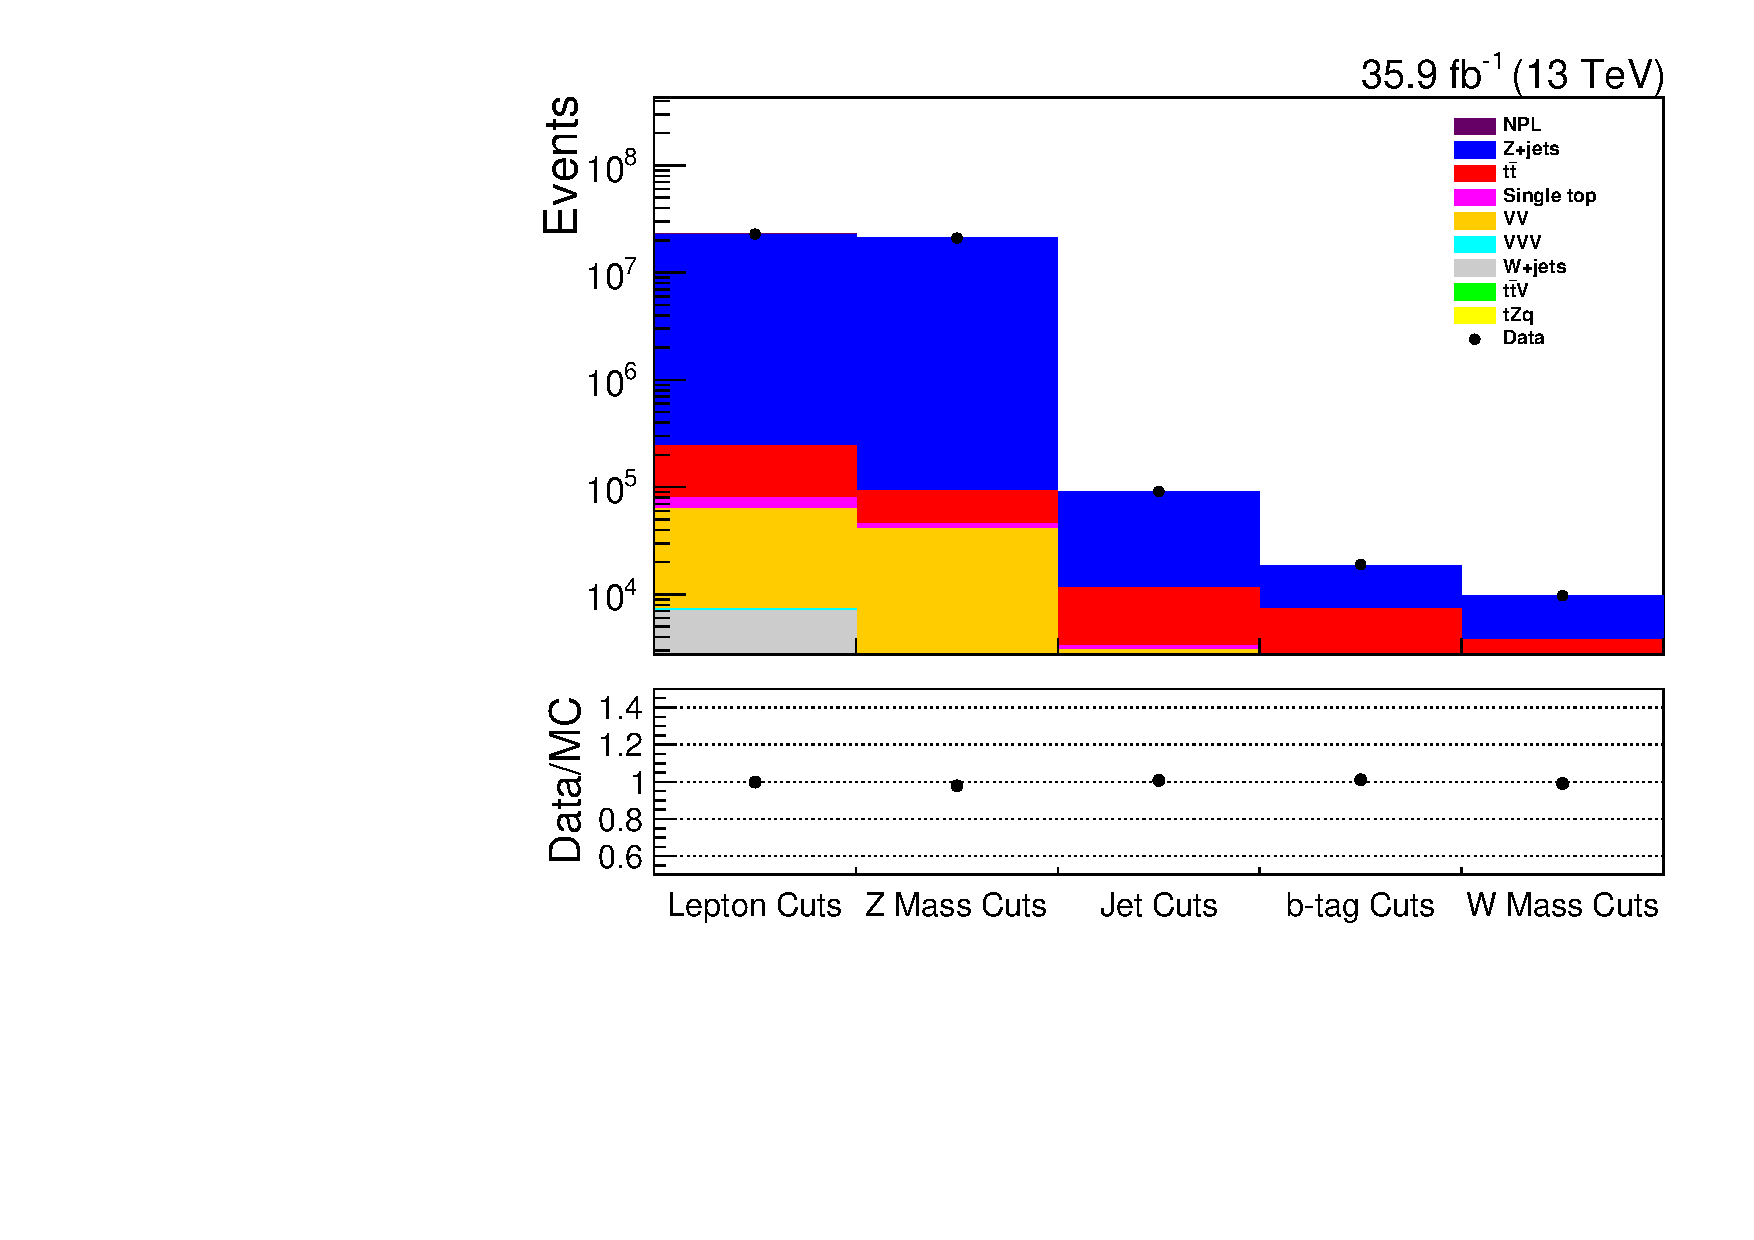
\includegraphics[width=0.47\textwidth]{figs/background-estimation/plots/unblinded/prompt_mumu_ttbarInc/cutFlow_log.pdf}
\\
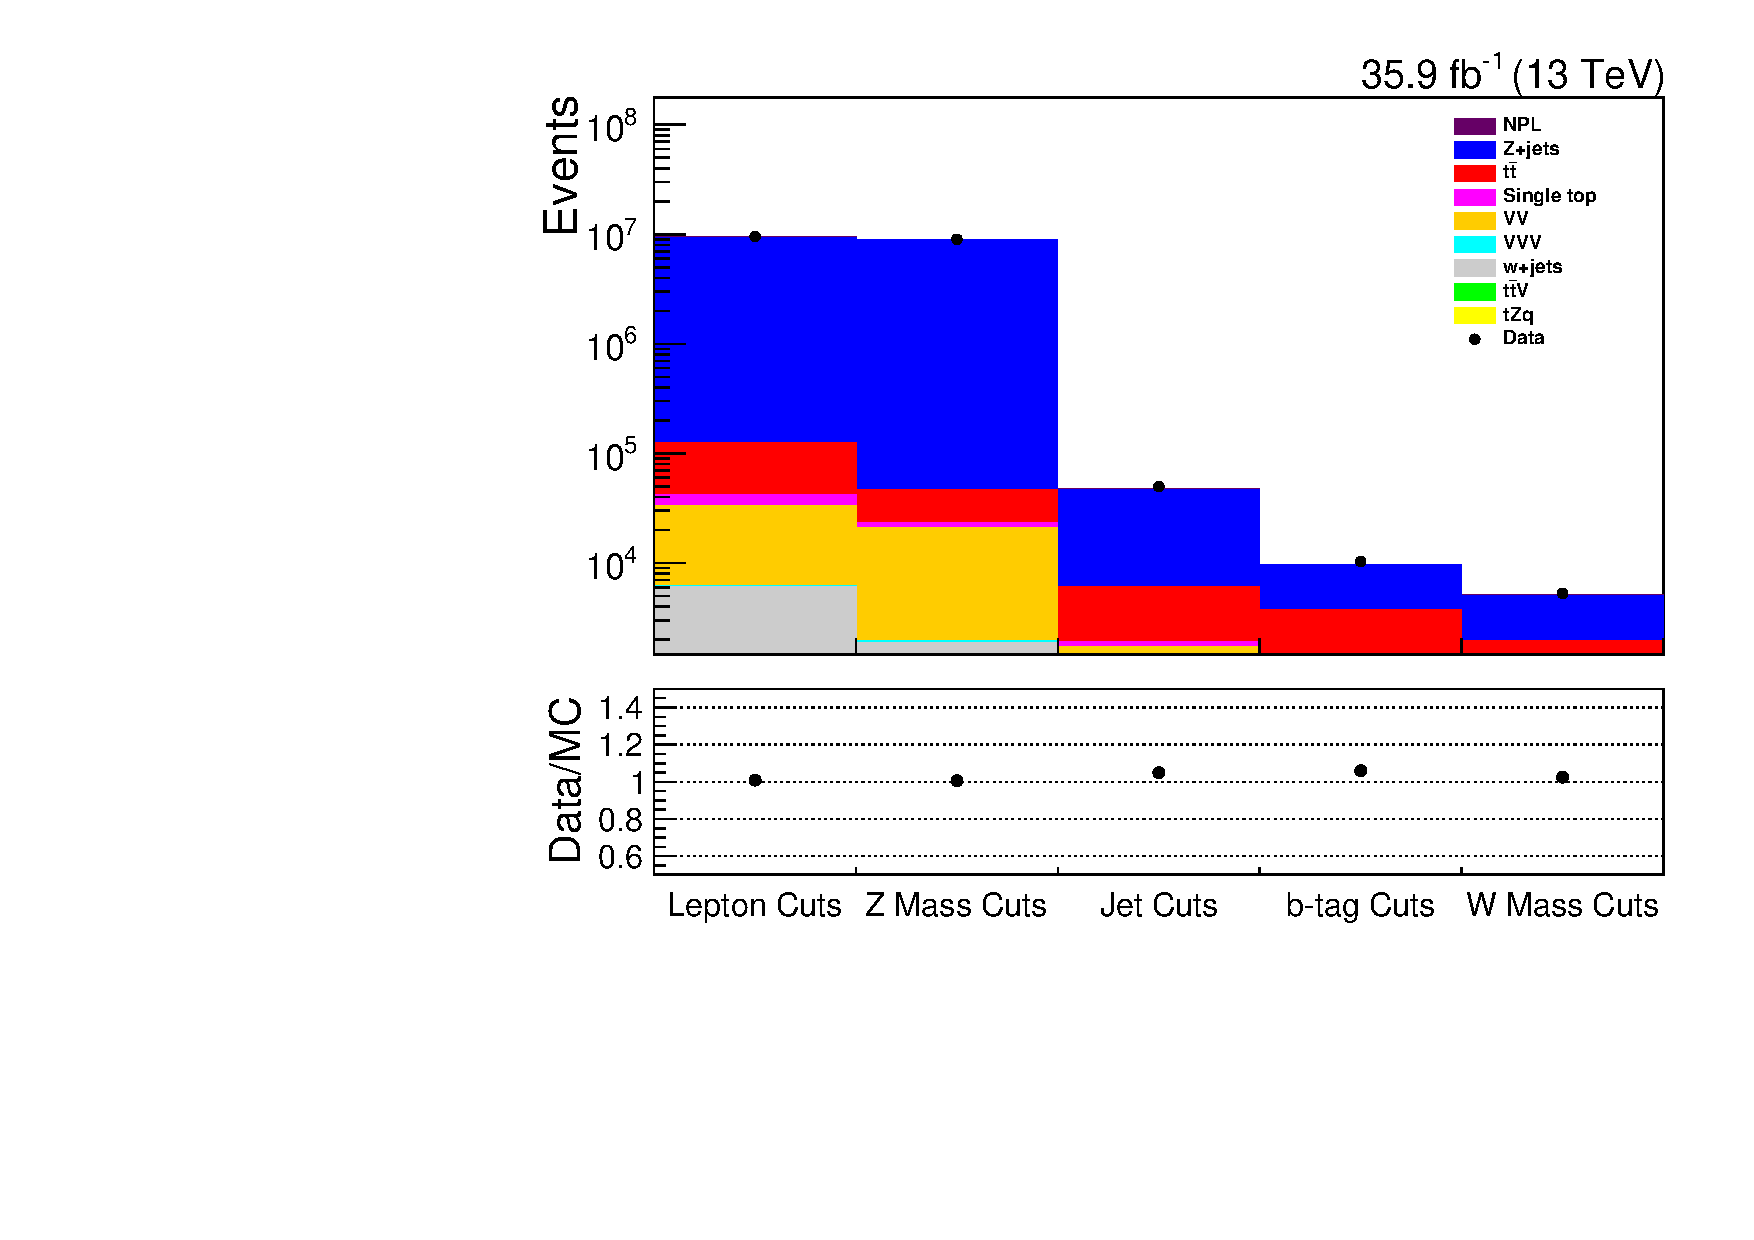
\includegraphics[width=0.47\textwidth]{figs/background-estimation/plots/unblinded/prompt_ee_ttbarInc/cutFlow_log.pdf}
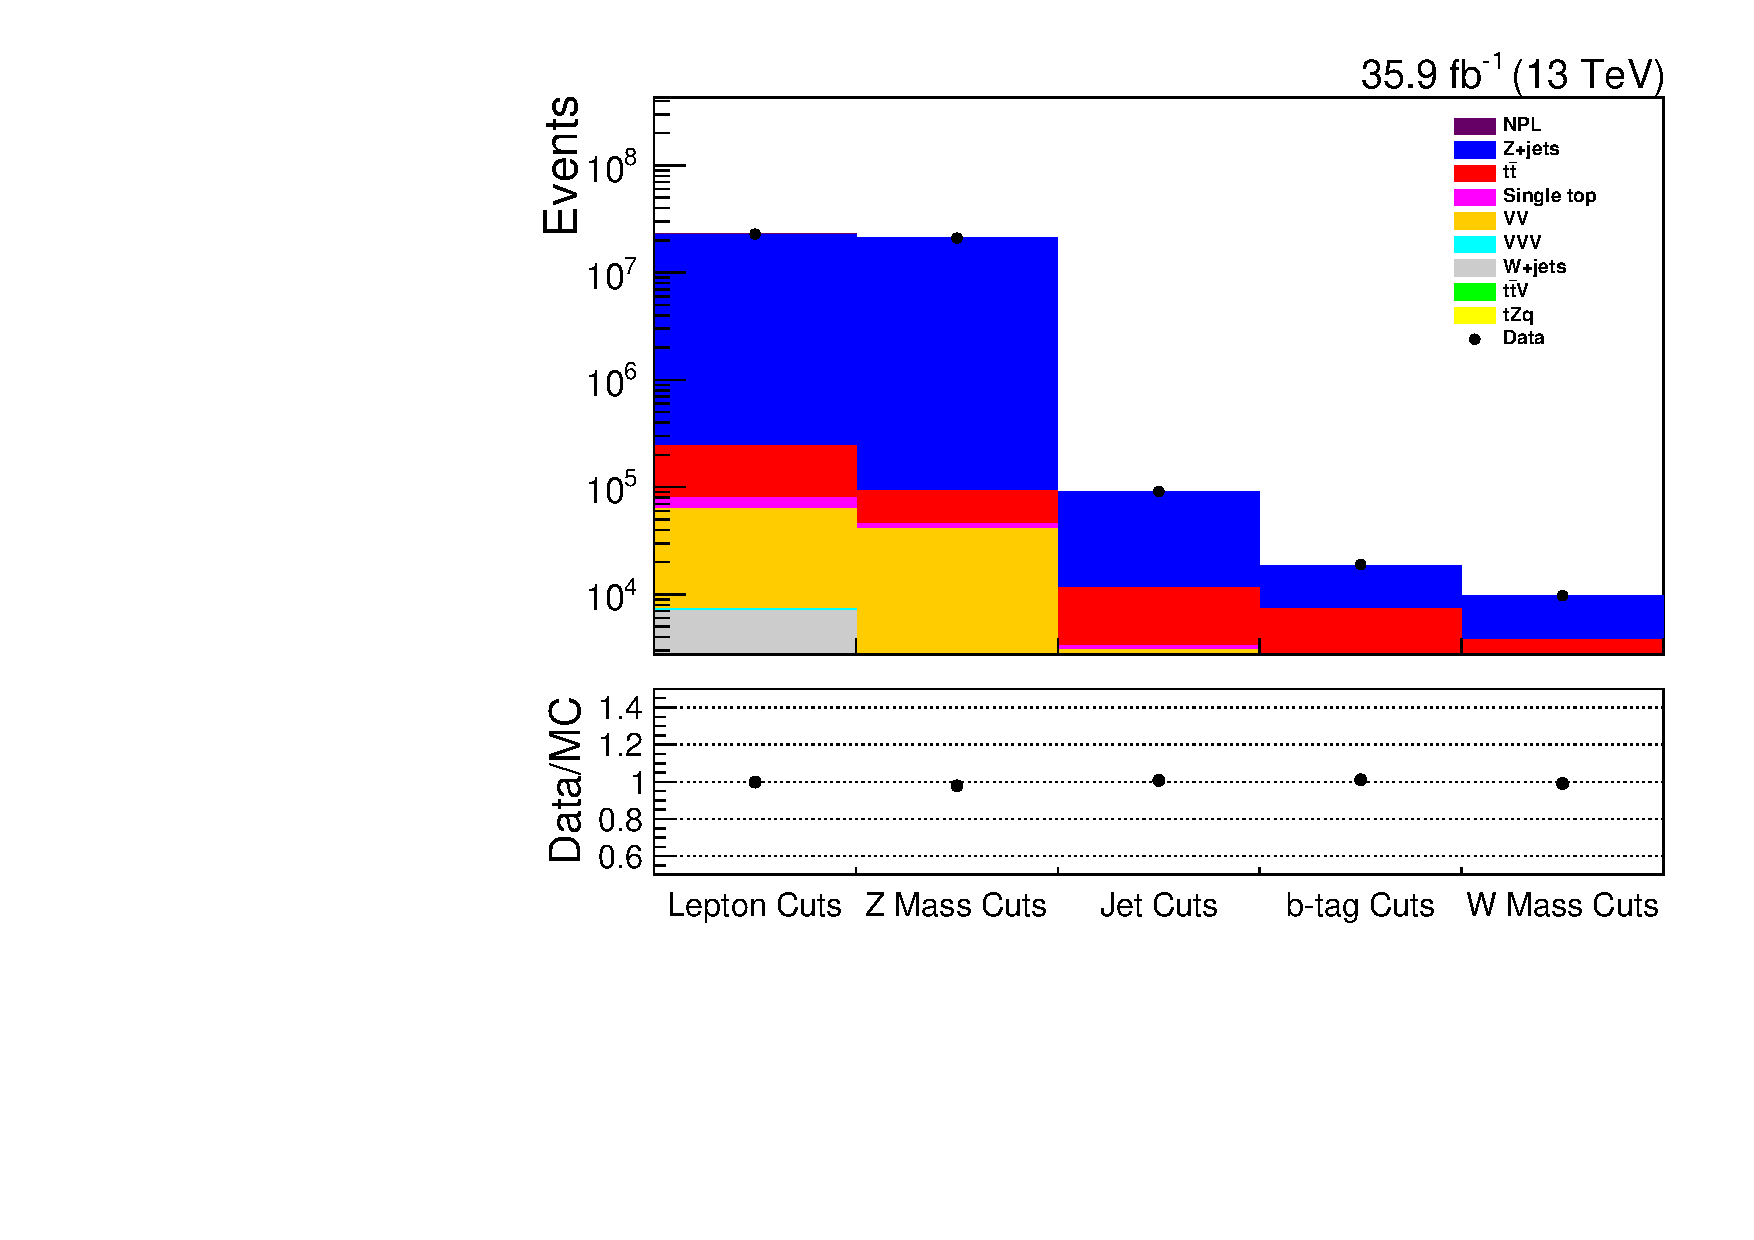
\includegraphics[width=0.47\textwidth]{figs/background-estimation/plots/unblinded/prompt_mumu_ttbarInc/cutFlow_log.pdf}
\caption{
The electron \pT (left) and $\eta$ following applying the lepton selection criteria (top) and the jet selection criteria (bottom).
}
\label{fig:ttbar_electron}
\end{figure}

\begin{figure}[h]
\centering
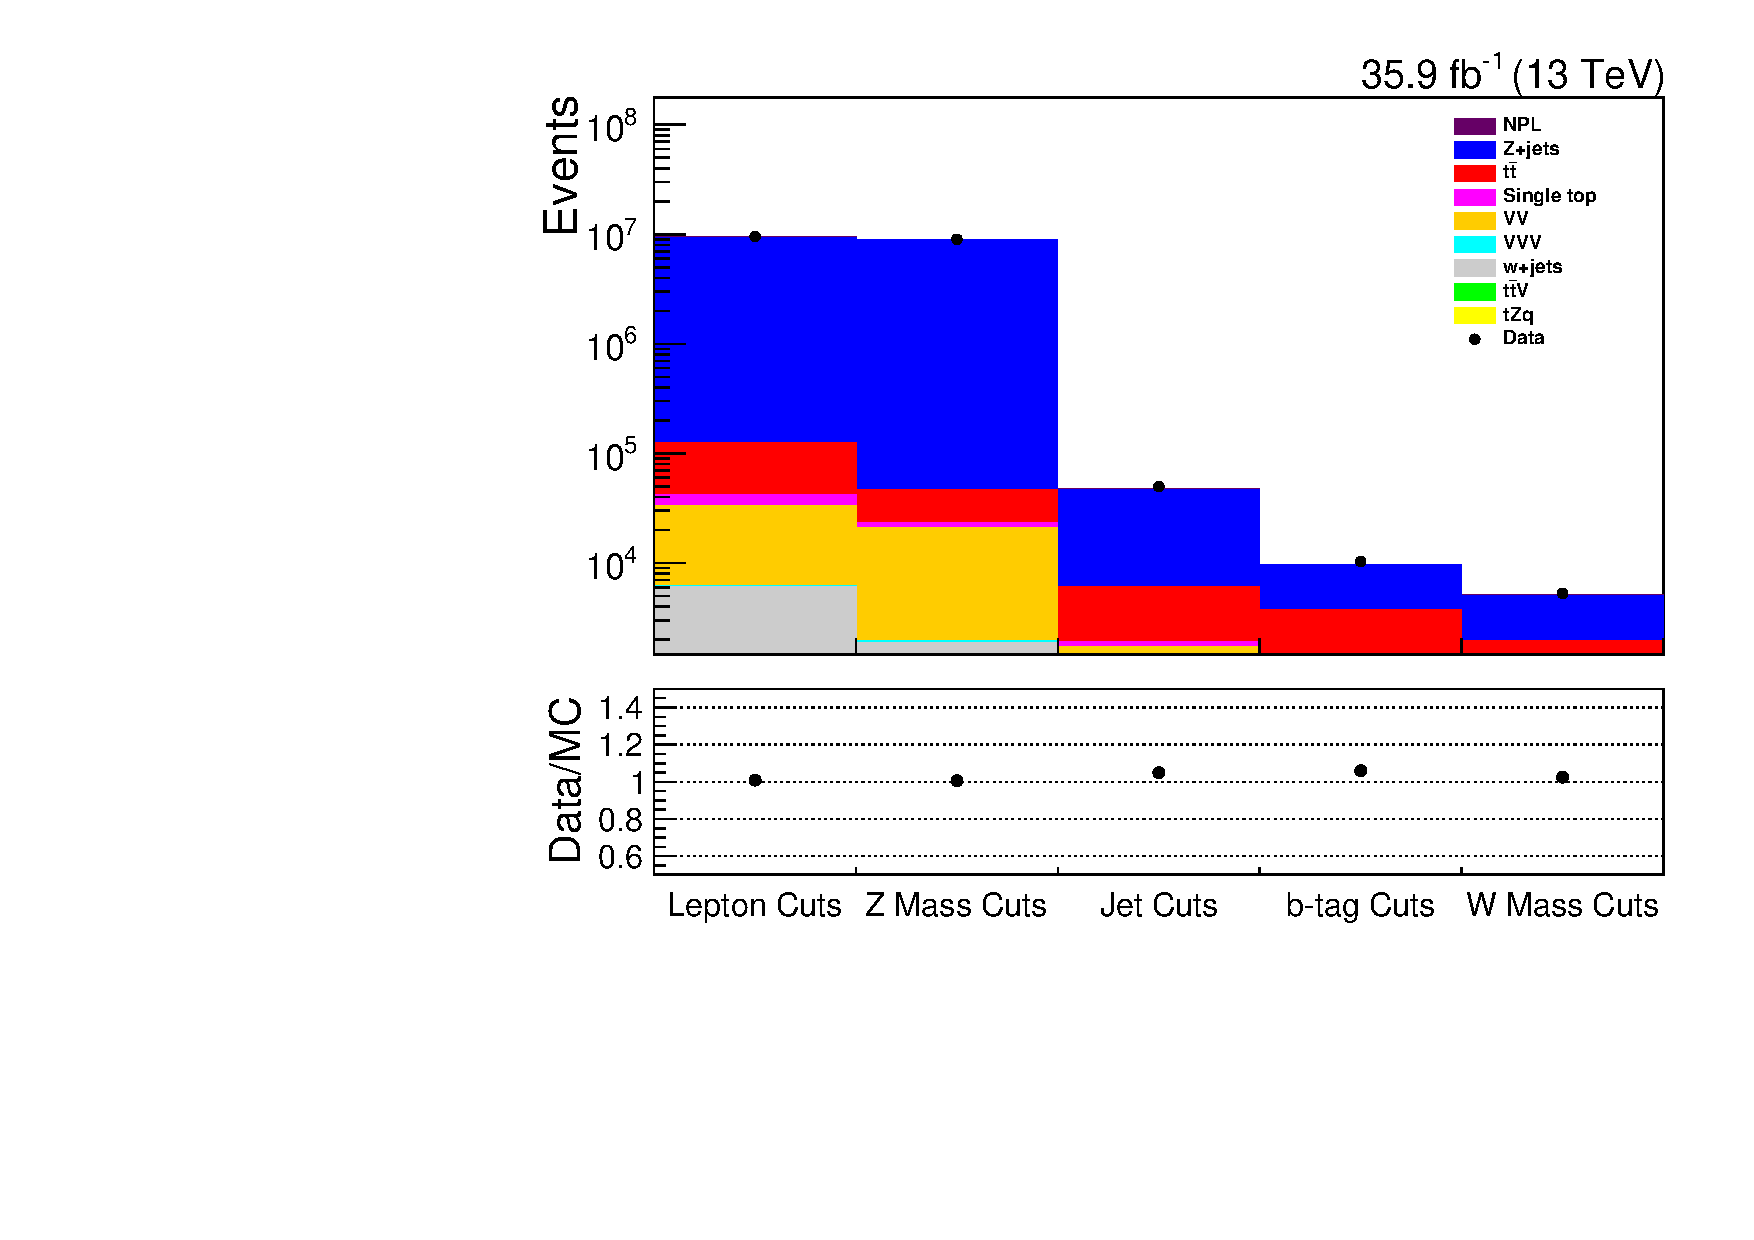
\includegraphics[width=0.47\textwidth]{figs/background-estimation/plots/unblinded/prompt_ee_ttbarInc/cutFlow_log.pdf}
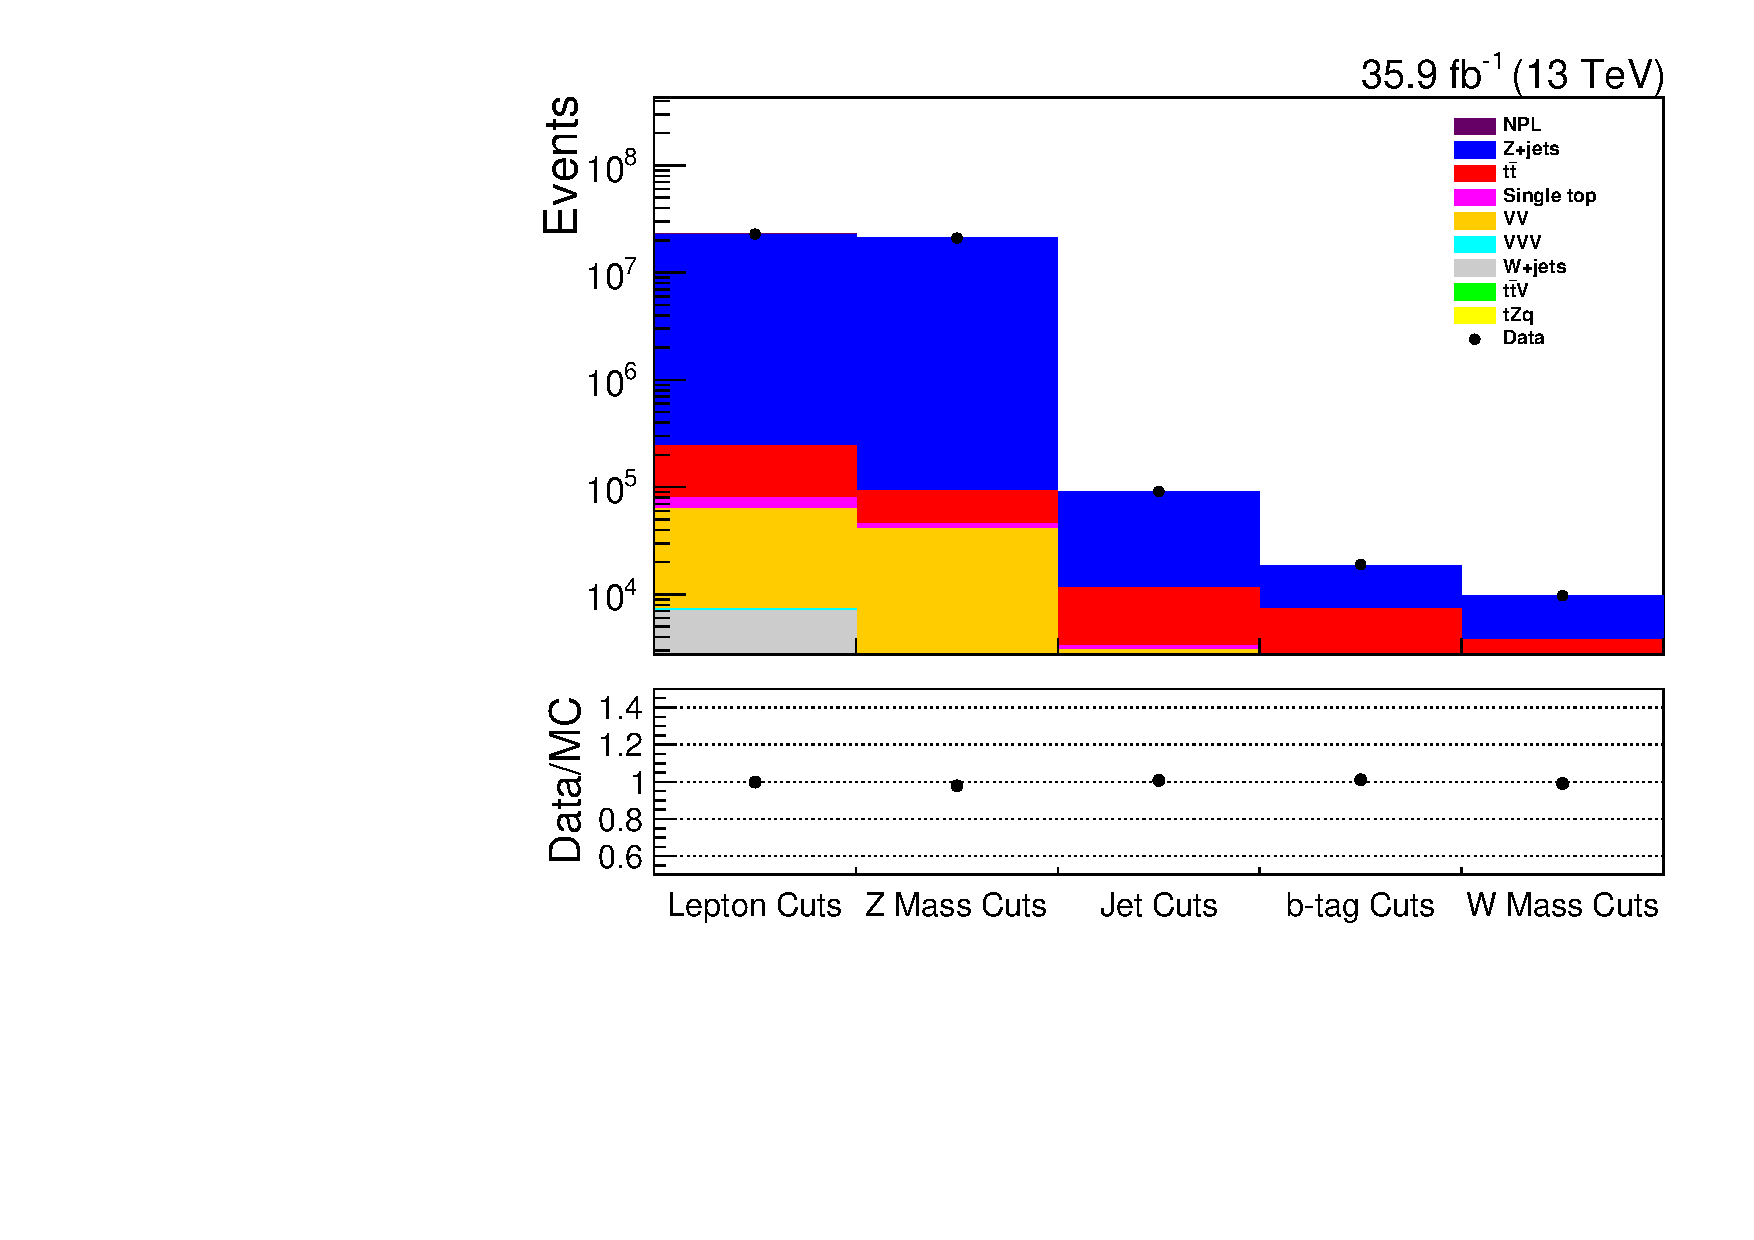
\includegraphics[width=0.47\textwidth]{figs/background-estimation/plots/unblinded/prompt_mumu_ttbarInc/cutFlow_log.pdf}
\\
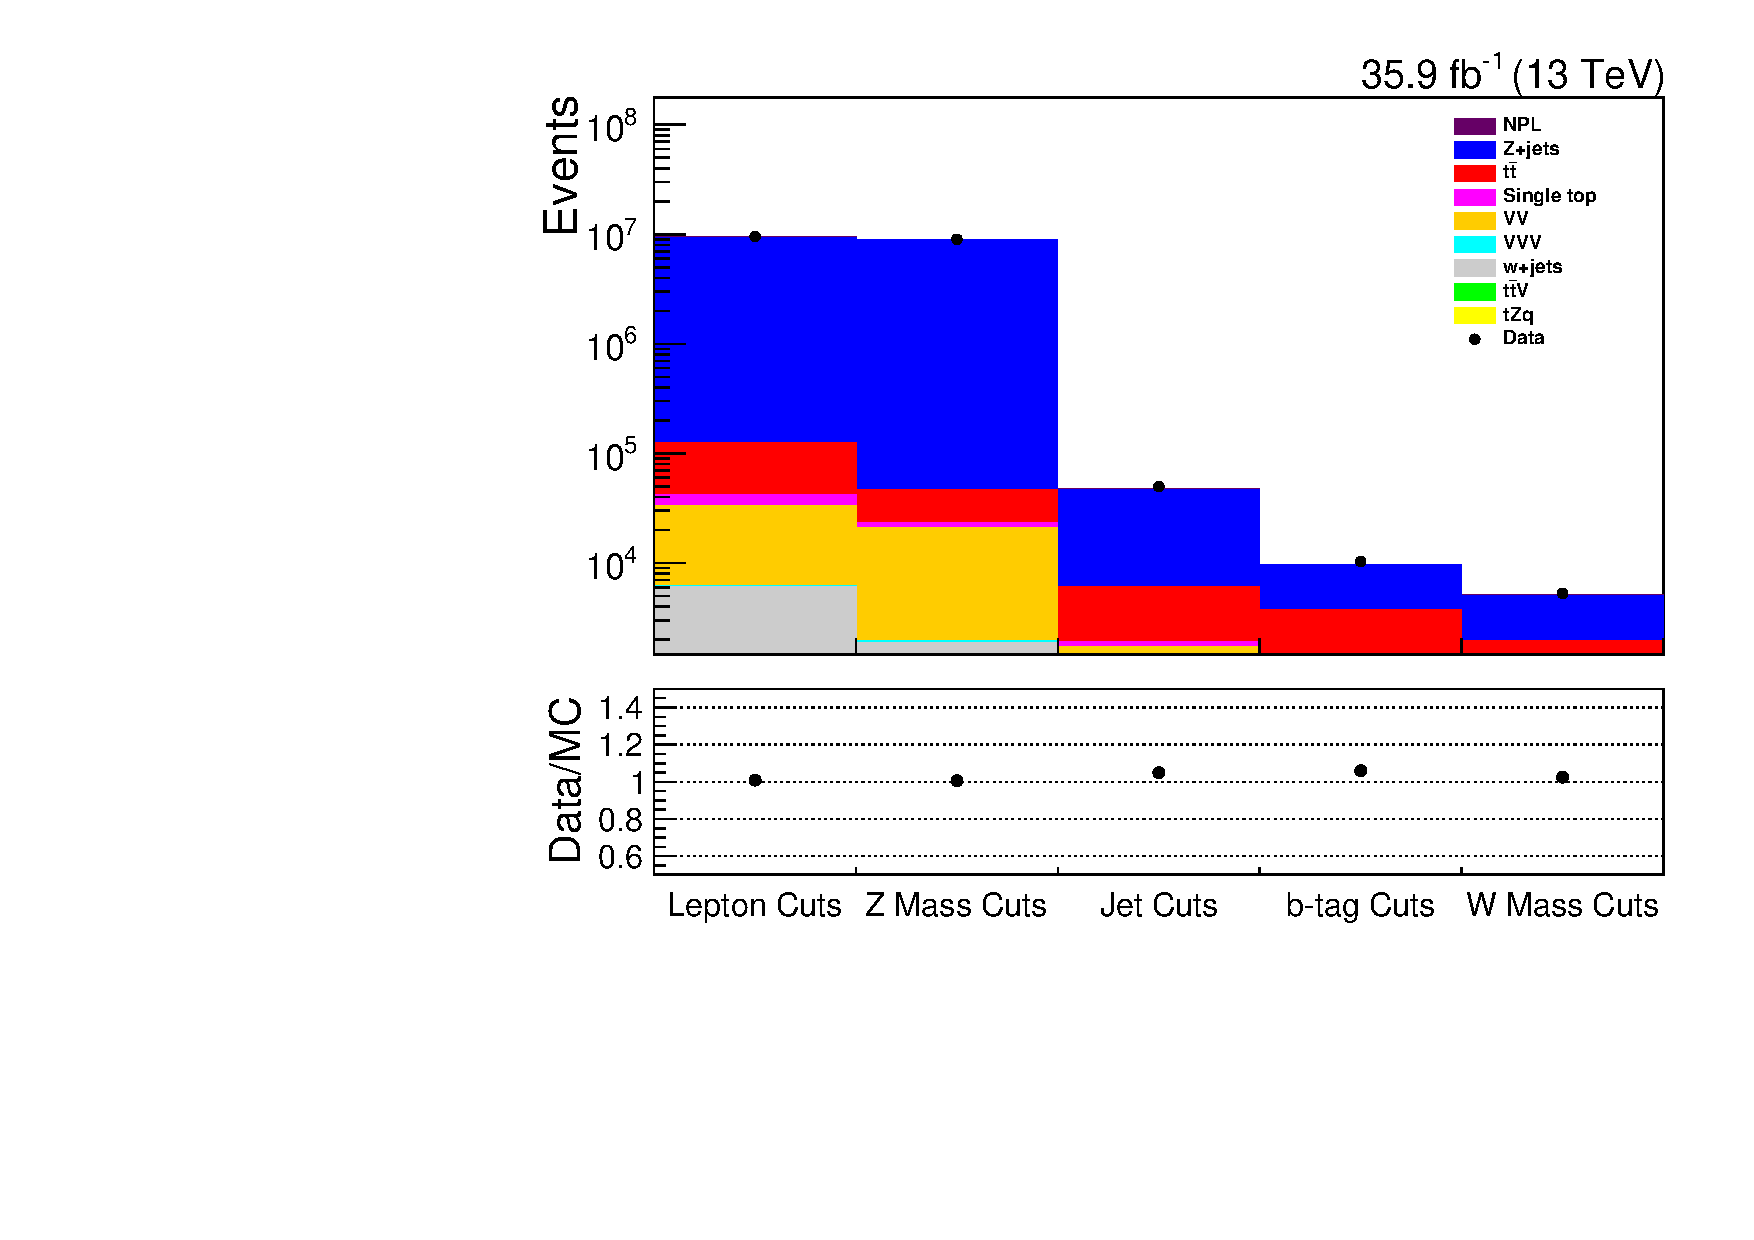
\includegraphics[width=0.47\textwidth]{figs/background-estimation/plots/unblinded/prompt_ee_ttbarInc/cutFlow_log.pdf}
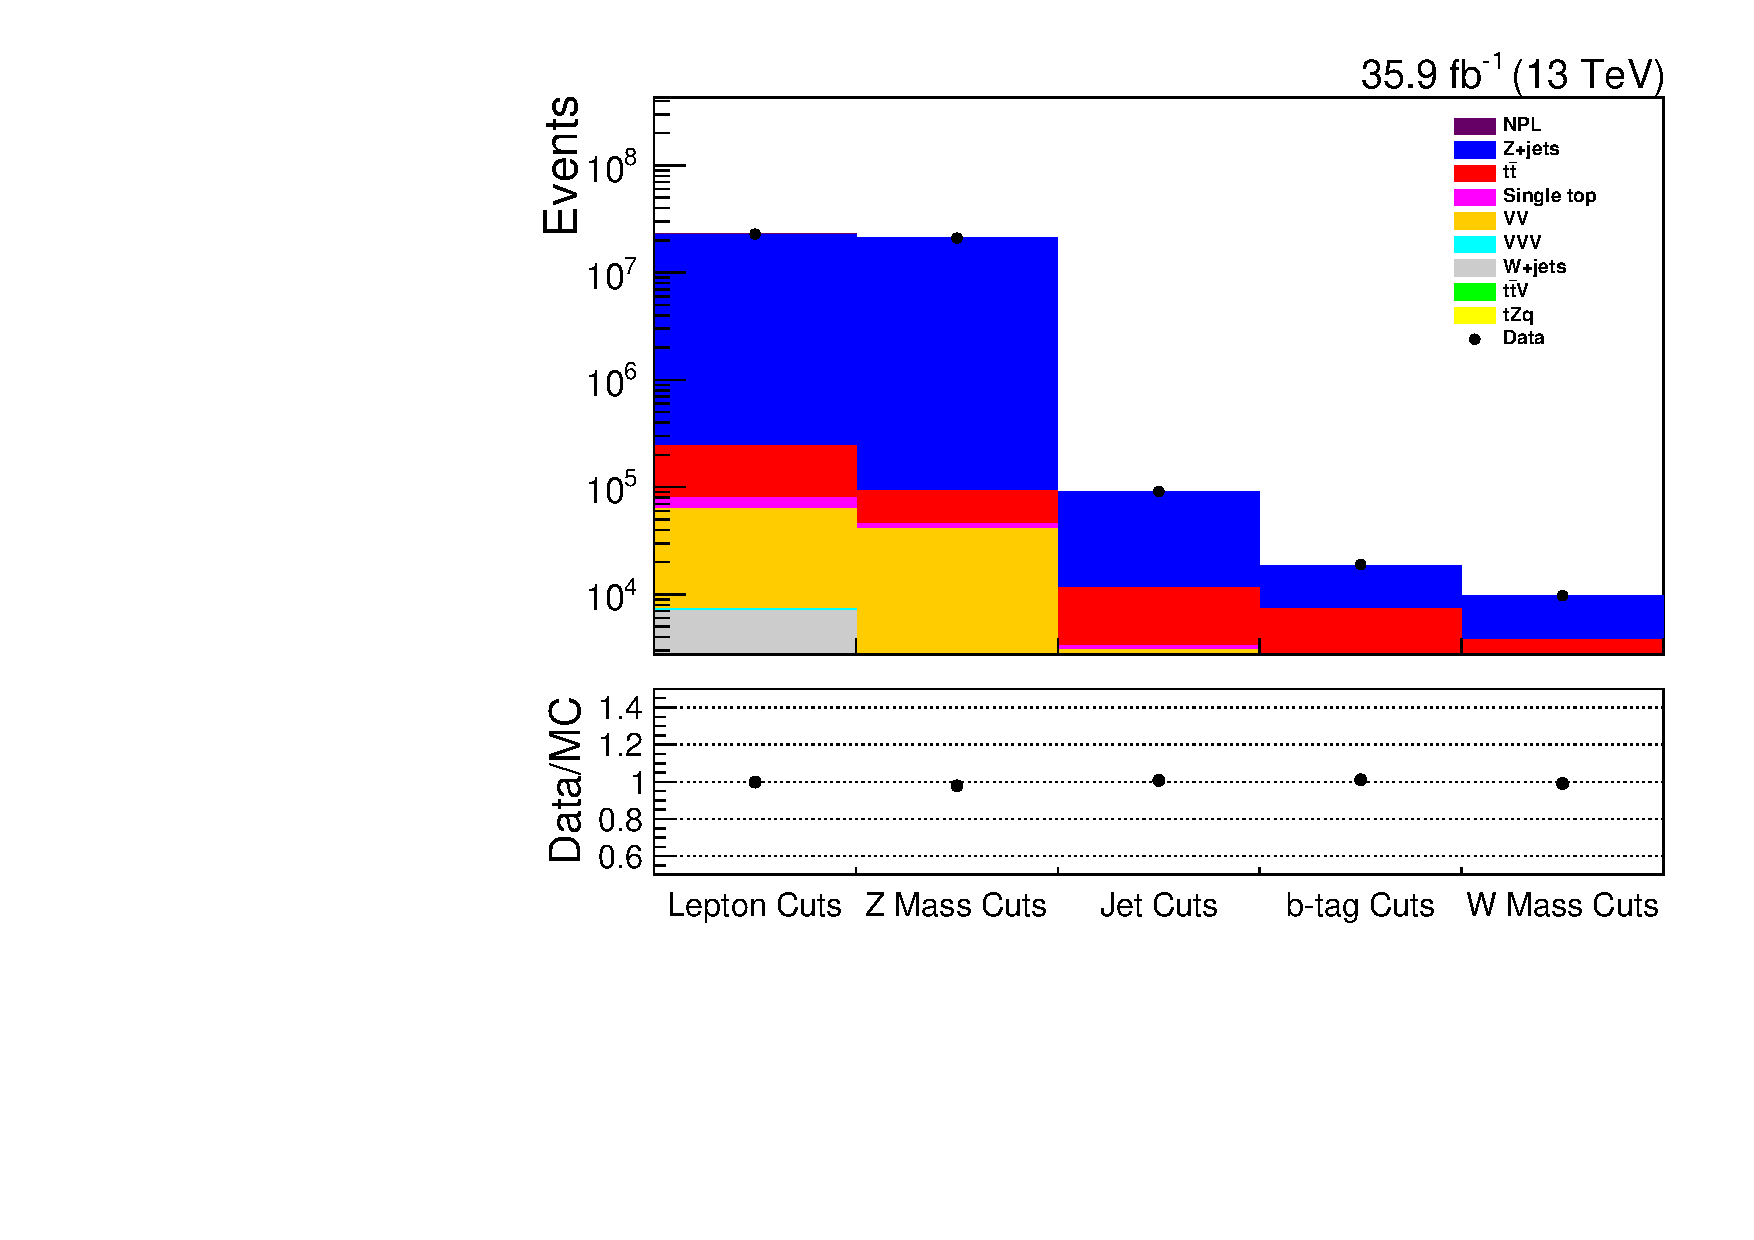
\includegraphics[width=0.47\textwidth]{figs/background-estimation/plots/unblinded/prompt_mumu_ttbarInc/cutFlow_log.pdf}
\caption{
The muon \pT (left) and $\eta$ following applying the lepton selection criteria (top) and the jet selection criteria (bottom).
}
\label{fig:ttbar_muon}
\end{figure}